\documentclass[10pt,a4paper]{article}
\usepackage[utf8]{inputenc} % para poder usar tildes en archivos UTF-8
\usepackage[spanish, es-tabla]{babel} % para que comandos como \today den el resultado en castellano
\usepackage{a4wide} % márgenes un poco más anchos que lo usual
\usepackage[conEntregas]{caratula}
\usepackage[table]{xcolor}
\usepackage{colortbl}
\usepackage{todonotes}
\usepackage{graphicx}
\usepackage{subcaption}
\usepackage{algorithm}
\usepackage{algorithmic}
\usepackage{dirtree}
\usepackage{cite}
\usepackage{listings}
\usepackage{multirow}
\usepackage{epsfig}
\usepackage[font=small,labelfont=bf]{caption}
\usepackage{verbatim}

\lstset { %
    language=C++,
    backgroundcolor=\color{green!5}, % set backgroundcolor
    basicstyle=\footnotesize,% basic font setting
}

%definations
\definecolor{Gray}{gray}{0.6}
\definecolor{ligthGray}{gray}{0.9}
\newcommand{\mc}[2]{\multicolumn{#1}{|c|}{#2}}

\hyphenation{UDP/IP}

\usepackage{verbatim}

\begin{document}

\titulo{NetworkDEVS}
\subtitulo{Una herramienta de estudio para modelar redes usando DEVS y PowerDEVS}

\fecha{\today}

\materia{Teoría de las telecomunicaciones}

\integrante{Belloli, Laouen Mayal Louan}{134/11}{laouen.belloli@gmail.com}

\maketitle

\tableofcontents
\newpage

\section{Introducción y Motivación}

El presente trabajo introduce un modelo DEVS de una red funcionando bajo el protocolo UDP/IP encuadrando lo mejor posible cada uno de sus módulos en su correspondiente capa respecto al modelo OSI presentado en la literatura oficial de la materia de teoría de la telecomunicaciones \cite{peterson2011computer}. El trabajo fue desarrollado en el simulador PowerDEVS y pensado como herramienta de estudio para futuros alumnos de la materia. \\

Además del modelo, este trabajo aporta un framework que permite programar y modificar los protocolos de una red de telecomunicaciones para luego simular su comportamiento y obtener feedback instantáneo de los resultados. También, usando el simulador PowerDEVS, se consigue brindar una interfaz gráfica intuitiva que mapea de forma directa los dispositivos de la red con los módulos del modelo. Esta interfaz gráfica permite crear distintos escenarios topológicos sin tener que tocar ni una linea de código. \\

Por otro lado, esta interfaz gráfica permite modularizar de forma explícita las distintas capas del modelo y sus interacciones. De esta forma, se programa cada protocolo en su capa correspondiente, esto no es menor, ya que si bien, teóricamente, los distintos protocolos están separados en capas y las redes pueden ser pensadas así, en la realidad, estas capas no existen de forma explicita y hay un salto entre las teorías de redes y los modelos en capas respecto de sus distintas implementaciones prácticas. Este modelo, permite a los alumnos hacer trabajos prácticos implementando los protocolos y manteniendo explicitas estas capas, por ende, permite acercar la teoría y la práctica de las redes de telecomunicaciones. \\

Si bien, el modelo realizado es un modelo DEVS (Discrete EVent System Specification), el mismo fue pensado para que no sea necesario más que una breve introducción al formalismo, por lo que mismo personas sin ninguna experiencia en DEVS deberían ser capases de poder utilizar el simulador, el modelo y el framework general propuesto en este trabajo. De todas formas, una explicación detallada sobre DEVS y PowerDEVS puede ser encontrada en \cite{bergero2011powerdevs}, un documento donde los autores de PowerDEVS explican con detalles, el formalismo DEVS y el simulador PowerDEVS. \\

\section{Objetivos}

Los objetivos de este trabajo se pueden dividir en varias partes:
\subsection{Desarrollar un framework para modelos de redes}

Como ya fue mencionado en la introducción, uno de los principales objetivos de este trabajo es desarrollar un framework, que permita fácilmente implementar protocolos de red, validarlos y experimentar con ellos mediante Simulación de Eventos Discretos (DES). Esta herramienta permite testear los protocolos implementados de forma sencilla y rápida. Obteniendo una herramienta útil, tanto para el estudio de las redes de telecomunicaciones como para la investigación en el área. 

La creación de un modelo que sirva como framework, tiene por objetivo factorizar y estandarizar las partes comunes a todos los protocolos, estás partes comunes provienen de las propiedades inherentes a los dispositivos físicos en los cuales los protocolos están corriendo, y de los estándares actualmente utilizados que permiten obtener robustez y compatibilidad entre distintas implementaciones que puedan existir en distintas partes de una red. Estas abstracciones encapsuladas en el modelo framework presentado, permiten al modelador, concentrarse plenamente en su protocolo y permite la reutilización y compatibilidad de distintos modelos que pueden luego ser combinados en un único modelo de una red que funcione bajo distintos protocolos, permitiendo así el estudio de la compatibilidad, homogeneidad y efectividad de los protocolos implementados.

\subsection{Modelar una red UDP/IP básica}

Por otro lado, este trabajo pretende implementar un modelo básico de una red UDP/IP que permita cubrir los protocolos mínimos e indispensables para permitir enviar mensajes entre distintos dispositivos. Este modelo no tiene como intensión implementar todas las partes, ni cubrir todos los protocolos, por lo que temáticas como la fragmentación de paquetes, congestión de tráfico, manejo de errores, Dinamic Host Configuration Protocol (DHCP) \cite[p.~231]{peterson2011computer}, Routing Information Protocol (RIP)\cite[p.~243]{peterson2011computer} y Spanning tree protocol \cite[p.~194]{peterson2011computer} quedan fuera del alcance de este trabajo, siendo los mismos posibles trabajos futuros. \\

También se implementó un modelo de switch que utiliza el protocolo Datagramas \cite[p.~172]{peterson2011computer} utilizando una forwarding table para enviar los Frames por la interface correspondiente. \\

Para completar el modelo, se implementó el protocolo DNS correspondiente a la capa de aplicación y se simuló un escenario en el cual un host desea obtener la dirección ip de otro host, cuyo dominio es network.devs.com.

\subsection{Mapeo entre el modelo UDP/IP y el modelo OSI}

En este trabajo, también pretendemos mostrar como se pueden implementar los distintos protocolos del modelo UDP/IP encuadrándolos en un modelo en capas OSI. Para esto, varias decisiones tuvieron que tomarse, siendo tal vez la más difícil, decidir en que capa implementar el protocolo ARP \cite[p.~228]{peterson2011computer}. Para tomar estas decisiones, se tomaron siempre como referencia los textos del libro oficial de la materia \cite{peterson2011computer}. Se intentó también separar lo mejor posible las tareas de cada capa de forma tal que cada una de ellas pueda ignorar lo más posible la existencia de la o las capas inferiores.

\section{Arquitectura}

\subsubsection{Conceptos básicos de la arquitectura}

La arquitectura general del modelo propuesto en este trabajo tiene por principal objetivo ofrecer un framework donde se pueda fácilmente desarrollar protocolos, para esto, se concentra en resolver varios puntos principales:

\begin{itemize}
\item Estandarizar la comunicación entre las capas de forma de conseguir consenso entre los distintos modeladores que usen esta herramienta, y que facilite una comprensión jerárquica y organizada del modelo entero para los lectores nuevos.
\item Implementar todas aquellas partes generales a todos los modelos de protocolos de forma que solo sea necesario concentrarse en el protocolo a implementar.
\item Minimizar lo más posible la necesidad de tener conocimientos avanzados sobre DEVS a la hora de utilizar la herramienta.
\end{itemize}

\newpage

\subsubsection{Arquitectura implementada}
La arquitectura consiste en un modelo acoplado ``dispositivo'' de $N$ capas, con $N > 0$ de forma que cada capa $i, i \in [1,..,N]$ se comunica con las capas $i+1$ e $i-1$ utilizando $8$ canales de comunicación distintos:

\begin{itemize}
\item Output port 0: Envío de datos a la capa $i+1$.
\item Output port 1: Envío de controles a la capa $i+1$.
\item Output port 2: Envío de datos a la capa $i-1$.
\item Output port 3: Envío de controles a la capa $i-1$.
\item Input port 0: Recepción de datos de la capa $i+1$.
\item Input port 1: Recepción de controles de la capa $i+1$.
\item Input port 2: Recepción de datos de la capa $i-1$.
\item Input port 3: Recepción de controles de la capa $i-1$.
\end{itemize}

Dado que no siempre sucede que en un dispositivo de la red, exista un solo módulo por capa, y dado que los puertos de salida y entradas están pensados para comunicarse con un solo modelo en la capa superior e inferior. Es necesario usar modelos demultiplexers que permitan redirigir los mensajes salientes por un puerto al modelo correspondiente de entre todas las posibles opciones. También, se puede usar modelos multiplexers para que los múltiples modelos de la capa superior o inferior envíen mensajes al modulo y quede guardado en el campo \textit{interfaz} la identidad del modulo de origen del mensaje si fuera necesario. \\

Ejemplos de estos son: 
\begin{itemize}
\item Un host que tiene varias aplicaciones enviando datos a través de distintos sockets: Hay más de un módulo en la capa de aplicación (capa siete del modelo OSI) de ese host.
\item  Un router que tiene más de una interfaz: Hay una interfaz por cada sub-red a la cual esté conectado, contando con más de un modulo en la capa de linkeo (capa dos del modelo OSI).
\end{itemize}

Las capas $1$ y $N$ usan la misma arquitectura que el resto de las capas y tienen definidos los mismos puertos. Como existe solo un medio de comunicación físico entre dispositivos por donde datos y controles son enviados, el modelo acoplado ``dispositivo'' tiene solo un puerto de salida y un puerto de entrada destinado a comunicarse con otros dispositivos, y queda en el modelador decidir que puerto o puertos de salida de la capa $1$ conectar con el puerto de salida del modelo acoplado y que puerto o puertos de entrada de la capa $1$ comunicar con los el puerto de entrada. Por otro lado, el input requerido por la capa $N$ (comunmente el input que indica los pedidos del usuario de enviar o recibir datos) se puede obtener mediante modelos generadores situados adentro del modelo acoplado. Lo mismo ocurre con el output generado por la capa $N$, este output puede ser recibido por modelos vertederos que lo guardan en archivos. \\

Distintos dispositivos de la red pueden tener distintas cantidades de capas, por lo cual, la cantidad de capas existente puede variar entre los distintos modelos de cada dispositivo dentro de una misma red. Los hosts por ejemplo, suelen tener hasta la capa siete, mientras que los routers comunes llegan a la capa tres y los switches a la capa dos. \\

La Figura \ref{figure:general architecture} muestra la arquitectura general recién explicada en un modelo de una red con un host y un router, en el mismo se pueden ver: los multiplexers y demultiplexers, modelos con distintas cantidades de capas y las conexiones entre capas utilizando los distintos puertos. \\

\begin{figure}[t]
    \centering
    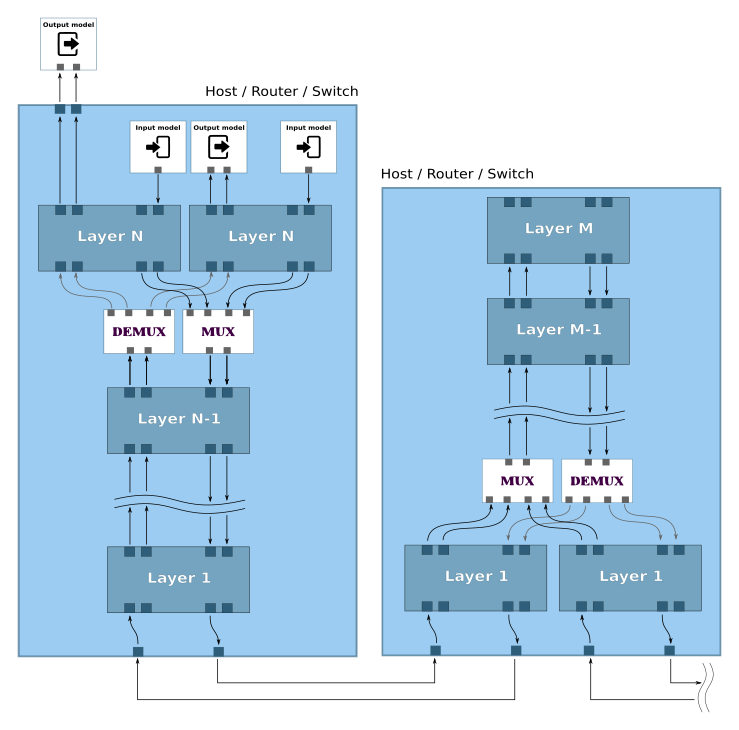
\includegraphics[width = 0.8\textwidth]{img/png/general_architecture.png}
    \caption{Arquitectura de un modelo en NetworkDEVS con dos dispositivos de N y M capas correspondientemente.}
    \label{figure:general architecture}
\end{figure}

\newpage

\subsubsection{Arquitectura de las capas}

La arquitectura de las capas está implementada en un modelo template llamado Layer del cual se puede realizar herencia para heredar su estructura. Esta estructura permite abstraer al protocolo de todo el modelo correspondiente al dispositivo, en otras palabras, esta estructura ya modela las propiedades de un dispositivo genérico, esto implica manejar el envío y recepción de mensajes a y desde las otras capas. Para manejar la entrada y salida de mensajes se utilizan colas FIFO; Cada vez que hay un mensajes entrante, el mismo es encolado en la cola de entrada correspondiente y el protocolo los va desencolando y atendiendo de uno o de a muchos dependiendo su implementación, el modelo template ya está armado de forma que mientras no haya mensajes por procesar se mantiene pasivado (en estado IDLE) y mientras que hay mensajes por procesar se queda ciclando para ir atendiéndolos a todos hasta que no halla más mensajes a procesar, momento en el que el modelo se vuelve a pasivar. Por otro lado, cada vez que se quiere enviar un mensaje, el mismo solo debe ser encolado en la cola de mensajes salientes correspondiente dependiendo de si es un mensaje de datos o control a la capa superior o inferior, luego el simulador cuando el protocolo termina el procesamiento actual se encarga de ciclar entre las colas de salida para enviar todos los mensajes que hallan sido encolados. La Figura \ref{figure:layer general architecture} muestra la arquitectura general de una capa cualquiera y la Figura \ref{figure:processing flow} muestra el flujo de procesamiento generado por el modelo template cuando es extendido agregándole un protocolo.

\begin{figure}[t]
    \centering
    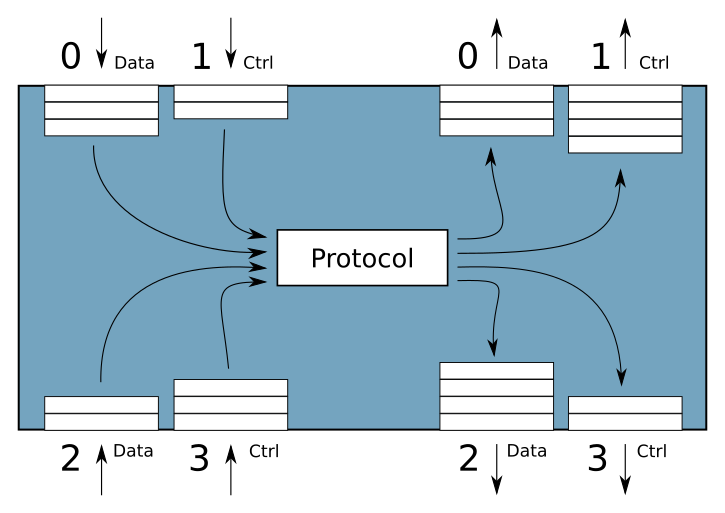
\includegraphics[width = 0.4\textwidth]{img/png/layer_architecture.png}
    \caption{Arquitectura de una capa en NetworkDEVS.}
    \label{figure:layer general architecture}
\end{figure}

\begin{figure}[t]
    \centering
    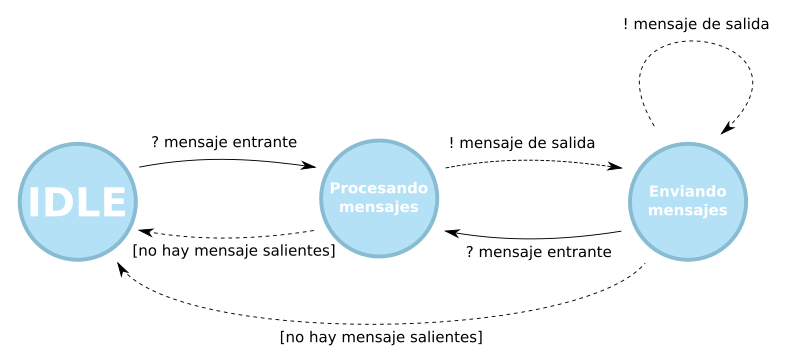
\includegraphics[width = 0.55\textwidth]{img/png/processing_flow.png}
    \caption{Flujo de procesamiento de una capa que extiende al modelo template Layer.}
    \label{figure:processing flow}
\end{figure}

\section{Como usar el template}

Todo el modelo está implementado en C++ y la forma de usar el template es mediante la implementación de herencias. Para poder comprender como utilizarlo, primero introduciremos la estructura de archivos del framework. \\

\dirtree{%
.1 NetworkDEVS.
.2 libs.
.3 logger.h.
.3 message\_queue.h.
.3 parser.h.
.2 structures.
.3 bastract\_types.h.
.3 ipv4.h1.
.3 mac.h.
.3 socket.h.
.2 templates. 
.3 layer.h.
.3 demultiplexer.h.
.3 multiplexer.h.
.3 input\_stream.h.
.3 output\_strem.h.
.2 LICENSE.
.2 README.md.
}

\medskip

La carpeta \textit{structures} es la que contiene las definiciones de todos los tipos de datos que vienen por defecto con el framework, algunos de ellos fueron implementados exclusivamente para el modelo presentado en este trabajo, pero todos pueden ser utilizados y están incluidos por el modelo template \textit{Layer} que introduciremos a continuación. Los tipos de datos están implementados usando structs y casi todos heredan de dos tipos abstractos definidos en \textit{abstract\_types.h} que sirven como organizadores. De esta forma quedan están separados entre los que son Data y los que son Headers. Cada tipo de dato definido cuenta con documentación en el código en formato Doxigen y la misma fue exportada y se encuentra disponible en el apéndice de este documento. \\

Todos los tipos de datos están implementados en namespaces que sirven como organizadores, para cada capa existente debe existir un namespace y los tipos de datos inherentes a esa capa tienen que estar definidos dentro del namespace (por más que otras capas lo usen). Si se implementan nuevas capas, se deben crear sus correspondientes namespaces a menos que no halla tipos de datos correspondientes a la capa. De está forma se evitan las ambigüedades que son muy recurrentes en el ámbito de las redes y se explicita la interacción con los datos correspondientes a cada capa. \\

\textbf{Note: } No están incluidos en esta estructura todos los archivos puntuales al modelo particular implementado, solo se encuentran aquellos archivos correspondientes a la arquitectura del framework. \\

\subsection{Como heredar el modelo layer}

El modelo \textit{Layer} es el modelo template que contiene toda la implementación correspondiente a la arquitectura general de una capa. El mismo es un modelo que cuenta con $4$ tipos de datos templates a instanciar y $4$ tipos de datos template con instanciación por defecto si no se explicitaran otros tipos para ellos. Estos tipos a instanciar son los tipos de los mensajes que envían y reciben los puertos y los tipos con los cuales se definen las colas. Por defecto se asume que los modelos intercambian los mismos tipos de datos, por ejemplo, si dos modelos intercambian datos de control, estos datos son del mismo tipo en ambas direcciones, sin importar quien es el que los envia y quien es el que los recibe. Es por esto que hay solo 4 tipos template que deben ser instanciados obligatoriamente, mientras que los restantes cuatro se mapean por defecto con los primeros 4. De todas formas, si se desea que los tipos de datos no sean iguales dependiendo quien envía y quien recibe, se pueden instanciar todos los tipos template.\\

El modelo \textit{Layer} tiene la siguiente forma:
\begin{lstlisting}
template <typename DH, CH, DL, CL, DH2 = DH, CH2 = CH, DL2 = DL, CL2 = CL>
class Layer: public Simulator { 

protected:
  // Logger
  Logger logger;

  // Colas de entrada
  std::queue<DH> higher_layer_data_in; // Input Port 0
  std::queue<DL> lower_layer_data_in;  // Input Port 1
  std::queue<CH> higher_layer_ctrl_in; // Input Port 2 
  std::queue<CL> lower_layer_ctrl_in;  // Input Port 3
  
  // Colas de salida
  message::queue<DH2> higher_layer_data_out = 0; // Output Port 0 
  message::queue<DL2> lower_layer_data_out = 1;  // Output Port 1
  message::queue<CH2> higher_layer_ctrl_out = 3; // Output Port 2
  message::queue<CL2> lower_layer_ctrl_out = 3;  // Output Port 3

  Event output;


  // Manipulacion del tiempo virtual de la simulacion 
  double next_internal;
  double last_transition;
  double infinity = std::numeric_limits<double>::max();
  bool queuedMsgs() const { ... }

public:

  Layer(const char *n): Simulator(n) {};
  double ta(
  Event lambda(double) { .... }
  void dint(double t) { .... }
  void dext(Event x, double t) { .... }
  
  virtual void dinternal(double t) {}
  virtual void dexternal(double t) {}
};
\end{lstlisting}

PowerDEVS tiene un par de exigencias a la hora de declarar un nuevo modelo, por este motivo, a continuación se muestra un ejemplo de herencia que puede ser usado de base para implementar nuevos modelos de capas. \\

\textbf{protocol\_name.h}
\begin{lstlisting}
//CPP:path_to_cpp_files/protocol_name.cpp
#include "template/layer.h"

class protocol_name: public Layer<T1, T2, T3, T4 [, T5, T6, T7, T8]> { 

protected:
	
  // Variables privadas del modelo
  // Metodos privados del modelo

public:
  protocol_name(const char *n): Layer(n) {};
  void init(double, ...);
  void exit();

  virtual void dinternal(double);
  virtual void dexternal(double);
  
  // Variables publicas del modelo
  // Metodos publicos del modelo
};
\end{lstlisting}

\textbf{Exigencias}
\begin{itemize}
\item La primer linea es requerida por el compilador de PowerDEVS y tiene que tener correctamente seteado la dirección al archivo \textit{.cpp} donde estén implementados todos los métodos del modelo.
\item El constructor de la clase debe estar declarado como se muestra en el ejemplo y la función \textit{init} es la utilizada por el simulador para inicializar el modelo. Esta función debe ser declarada como se muestra con los ``\ldots'' como parámetro, el simulador llama a esta función pasándole como primer parámetro \textit{double} la cantidad de parámetros a leer y luego el resto de los parámetros definidos para el modelo en la IDE PowerDEVS, los mismos se recuperan utilizando la librería \textit{va\_start} y \textit{va\_arg} \cite{vastart} \cite{vaarg}.
\item El método exit también debe ser declarado y el mismo es llamado por el simulador al finalizar la simulación. Todos los destructores correspondientes deben ser llamados en esta función de forma de liberar correctamente la memoria (de ser necesario).
\item El nombre de la clase debe estar escrito todo con minúsculas.
\end{itemize}

Como se puede observar existen las funciones \textit{dint} y \textit{dext} que son las funciones exigidas por el simulador para ejecutar correctamente las transiciones interna y externa correspondientes al formalismo DEVS, el modelo Layer ejecuta en esas funciones todo el código relativo a la arquitectura presentada y llama a los métodos virtuales \textit{dinternal} y \textit{dexternal} que son sobre escritos por el modelador para ejecutar el protocolo implementado. De esta forma se consigue abstraer lo más posible al modelador del formalismo, convirtiendo esta herramienta en una herramienta viable para el uso dentro del ámbito de estudio. \\

Por otro lado, la variable \textit{next\_internal} definida en en el template Layer es utilizada por el modelo para agendar la próxima transición interna. Si el protocolo no asigna ningún valor a esta variable, se asume que el protocolo tomó infinito tiempo en procesar y el modelo quedará pasivado hasta que llegué nuevos mensajes externos. Una vez que se cumple el \textit{next\_time}, el output correspondiente es inmediatamente enviado y luego el simulador queda pasivado a menos que haya más mensajes externos a procesar. El desarrollador del protocolo tiene que asignar en esta esta variable un modelo del tiempo de computo del protocolo para de esta forma modelar los tiempos reales de runtime\footnote{Una opción es medir el tiempo real de procesamiento mediante librerias c++ para asignar el valor real de tiempo de computo.}. Esta variable es de tipo double y la representación del tiempo mediante doubles queda en manos del modelador y debe ser consensuada con el resto de los modeladores de los demás protocolos para poder unirlos en un solo modelo, un consenso común es asumir que una unidad de double representa un segundo y utilizarlo de forma similar a los timestamps. \\

\subsection{Como enviar y recibir mensajes entre las capas}

Todos los mensajes que llegan al modelo de una capa son recibidas por uno de los cuatro siguientes puertos dependiendo de donde provenga el mensaje:
\begin{itemize}
\item std::queue$<DH>$ higher\_layer\_data\_in:  Input Port 0
\item std::queue$<DL>$ lower\_layer\_data\_in:   Input Port 1
\item std::queue$<CH>$ higher\_layer\_ctrl\_in:  Input Port 2 
\item std::queue$<CL>$ lower\_layer\_ctrl\_in:   Input Port 3
\end{itemize}

La Figura \ref{figure:layer general architecture} Muestra de que capa proviene y para que tipo de datos está pensado cada uno de estos puertos. \\

Como ya fue mencionado y como se puede observar en la definición de las colas, los tipos template instanciados son los tipos de los mensajes recibidos desde las capas superior e inferior. Es importante que los mensajes recibidos sean efectivamente de este tipo, porque el simulador PowerDEVS envía mensajes como \textbf{void *} y los mismos son casteados a su tipo correspondientes una vez recibidos por el modelo receptor, por lo que si los tipos no corresponden se generará un excepción en tiempo de ejecución. \\

Para procesar los mensajes, dentro del método \textit{dinternal}, los mismos deben ser desencolados, es importante que se desencolen, ya que en caso contrario el mismo seguirá estando en la cola y el modelo volverá a producir una transición interna y llamar de nuevo al método \textit{dinternal} procesando dos o más veces el mismo mensaje. Reprocesar un mensaje múltiple veces probablemente esté mal, pero tal vez es lo deseado por el protocolo, pero hay que tener en cuenta que una de las pocas exigencias del formalismo DEVS es que no ocurran infinitos eventos en un mismo momento del tiempo virtual, y como el modelo sigue generando transiciones internas mientras haya mensajes por procesar, si los mensajes no son nunca desencolados y la variable \textit{next\_internal} se mantiene en cero, se generan infinitas transiciones internas y eso produciría un modelo DEVS ilegítimo que cuelga al simulador. \\

\newpage

Para enviar mensajes las colas a utilizar son las siguientes:
\begin{itemize}
\item message::queue$<DH2>$ higher\_layer\_data\_out: Output Port 0 
\item message::queue$<DL2>$ lower\_layer\_data\_out:  Output Port 1
\item message::queue$<CH2>$ higher\_layer\_ctrl\_out: Output Port 2
\item message::queue$<CL2>$ lower\_layer\_ctrl\_out:  Output Port 3
\end{itemize}

Como se puede observar, los nombres de los tipos a instanciar son iguales a los de las colas de entrada con un $2$ al final, esto es porque los mismos por defecto se instancian usando los tipos de las colas de entrada a menos que en la declaración de la herencia se especifique lo contrario, esto es así ya que se considera buena práctica que el tipo de datos que intercambian dos capas por un canal de comunicación sea siempre el mismo en ambas direcciones, facilitando la reutilización y comprensión de los modelos por parte de otras personas, sin embargo esto no es siempre posible, principalmente cuando se interactua mediante modelos \textit{demultiplexers}. \\

Para encolar un mensaje en la cola de salida correspondiente se debe utilizar el método \textit{message::queue::push(MSG mensaje)}. De la misma forma que el modelo Layer se encarga de encolar los mensajes en la cola de entrada correspondiente dependiendo el puerto por donde llegó el mensaje, el mismo se encarga de desencolar y enviar los mensajes encolados en las colas de salidas por el puerto correspondiente a cada cola y desencolar el mismo. \\

El tipo de datos message::multiplexed$<typename MSG>$ sirve para enviar mensajes que van a ser demultiplexados por un modelo demultiplexer$<typename MSG>$. El mismo cuenta con los campos \textit{message} e \textit{interface} que son utilizados para asignar el mensaje y el identificador del destinatario. Luego solo resta utilizar un modelo demultiplexer, setear correctamente sus parámetros en la IDE de PowerDEVS\footnote{Para setear parámetros en un modelo hay que hacer clic derecho -$>$ parameters}, y conectar correctamente sus puertos de entrada y salida con el modelo de origen y los modelos de destino, la Tabla \ref{table: parameter demultiplexer} explica los parámetros a setear en estos modelos. La Figura \ref{figure: demultiplexer} muestra como es el mapeo de los puertos de un demultiplexer conectado a \textit{k} modulos\footnote{En el modelo implementado en este trabajo hay ejemplos de como utilizar el modelo demultiplexer con el tipo de dato message::multiplexed}\footnote{Un demultiplexer con relación $1$ a $k$ numera los módulos de salida de $0$ a $k-1$}. \\

\begin{table*}[h]
	\begin{tabular}{|l|c|c|c|}
  		\hline
  		\textbf{Nombre} & \textbf{Tipo} & \textbf{Descripción} \\
  		\hline
  		Module\_name & String & El nombre del módulo que utiliza el logger \\
  		\hline
  		Max\_interface & Int & La cantidad máximas de interfaces de salida que puede demultiplexar. \\
  		\hline
	\end{tabular}
	\caption{Parámetros del modelo demultiplexer}
	\label{table: parameter demultiplexer}
\end{table*}

\begin{figure}[t]
    \centering
    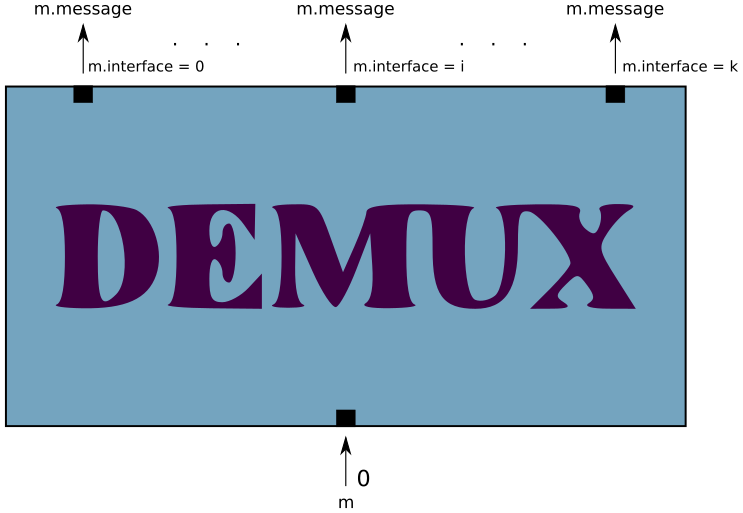
\includegraphics[width = 0.6\textwidth]{img/png/demultiplexer.png}
    \caption{Puertos de entrada y salida de un demultiplexer, mapeo del campo interfaz del mensaje con el puerto de salida correspondiente.}
    \label{figure: demultiplexer}
\end{figure}

El campo \textit{interface} le indica al demultiplexer por que puerto enviar el mensaje, por lo que es importante conectar correctamente los puertos de salida del demultiplexer con los puertos de entrada de los destinatarios, la entrada de mensages del modelo $i$ de destino debe estar conectado al puerto de salida $i$ del demultiplexer, la Figura \ref{figure: demultiplexer} muestra el mapeo de puertos de un demultiplexer. \\

\newpage

\subsection{Como implementar el protocolo de una capa (internal/external functions)}

El template cuenta con dos métodos virtuales que están definidos e implementados como funciones vacías (sin comportamiento), estos métodos son los que deben ser sobre escritos para implementar el protocolo. Siempre que haya mensajes por procesar en las colas de entradas, el modelo llama al método \textit{dinternal} en el cual se deben procesar dichos mensajes, el modelo Layer mira las colas de salidas para ver si hay mensajes a enviar y los envía, si al finalizar este proceso sigue habiendo mensajes por procesar en la cola de entrada se volverá a llamar a esta función respetando el formalismo DEVS de forma de seguir procesando mensajes. Este ciclo se repite indefinidamente hasta que no haya mas mensajes por procesar, momento en el cual el modelo se pasiva a la espera de nuevos eventos externos. \\

El método virtual \textit{dexternal} existe por si se desea implementar código que se ejecute cada vez que ocurre un evento externo para modificar el estado de las variables internas del protocolo o por algún otro motivo. Esto no es recomendado para desarrolladores no familiarizados con el formalismo DEVS o con el simulador PowerDEVS. \\

\section{Como agregar una capa}

Hay dos tipos de modelos: los modelos atómicos y los modelos acoplados. Para implementar un modelo de capa, primero es necesario heredar del template Layer para obtener el modelo atómico capa como fue descripto en la sección anterior y luego el mismo debe ser insertado mediante la IDE PowerDEVS dentro del modelo acoplado de un dispositivo, luego en el \textit{TOP model} se interconectan todos los modelos acoplados de los dispositivos. \\

Como se muestra en la arquitectura general, las capas deben ser insertadas dentro de los modelos acoplados de dispositivos (hosts, switches, routers, etc), por lo que antes de agregar la capa al modelo hay que abrir el modelo acoplado dispositivo en caso de existir, o crear el modelo acoplado dispositivo en caso de todavía no existir.

\begin{itemize}
\item \textbf{Abrir un modelo acoplado en PowerDEVS:} Seleccionar con el mouse el modelo acoplado a abrir y desplegar el menú de opciones del mismo dando click derecho sobre el icono, luego elegir la opción ``open model''.
\item \textbf{Crear un modelo acoplado en PowerDEVS: } Abrir la pestaña ``Basic Elements'' del sector ``library'' de la IDE y arrastrar el icono ``Coupled'' desde el menú hasta el sector donde esta el dibujo del modelo.
\end{itemize}

La figura \ref{figure: PowerDEVS IDE} muestra la IDE PowerDEVS e indica como crear un modelo acoplado dentro de la misma. \\

\begin{figure}[htbp]
    \centering
    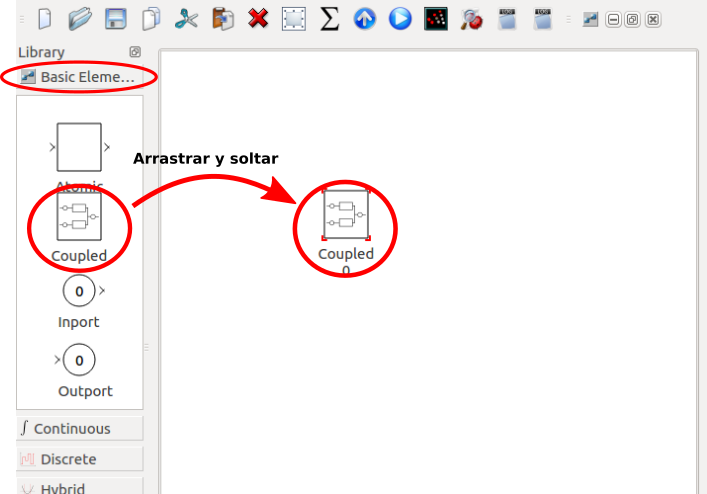
\includegraphics[width = 0.6\textwidth]{img/png/powerDEVS_coupled.png}
    \caption{Screenshot de la IDE PowerDEVS con la pestaña ``Basic Elements'' abierta resaltando el icono de coupled model.}
    \label{figure: PowerDEVS IDE}
\end{figure}

Para insertar un nuevo modelo de capa dentro de un modelo acoplado de dispositivo en PowerDEVS hay que seguir los siguientes pasos:

\begin{enumerate}
\item Crear el modelo acoplado de dispositivo (en caso de ser necesario) y abrirlo.
\item Crear un nuevo modelo atómico de capa:
\begin{enumerate}
\item De la solapa ``Basic Elements'' arrastrar al escenario el icono ``atomic''.
\item Click derecho sobre el icono del nuevo modelo atómico en el escenario.
\item Elegir la opción  ``edit''.
\item Ir a la pestaña ``code'', navegar por los modelos hasta encontrar el archivo \textit{.h} del modelo capa creado y seleccionarlo.
\item Ir a la pestaña ``parameters'' y agregar todos los parámetros requeridos por el modelo, o sea aquellos que el simulador le va a pasar al método ``init'' del modelo para inicializarlo y que serán leídos usando \textit{va\_arg} \footnote{Estos parámetros dependen de la implementación particular del protocolo.}.
\item Ir a la pestaña ``properties'' y realizar las siguientes tareas: Escribir el nombre deseado para el nuevo modelo, setear cuatro puertos de entrada y cuatro puertos de salida y elegir el icono a mostrar en el modelo (Elegir un icono no es obligatorio)
\end{enumerate}
\item Conectar las salidas de los modelos superiores e inferiores con las entradas del nuevo modelo según lo explicado anteriormente en la sección \textit{Como enviar y recibir mensajes entre las capas}.
\item Conectar las salidas del nuevo modelo a las entradas correspondientes de los modelos de las capas superiores e inferiores según lo explicado anteriormente en la sección \textit{Como enviar y recibir mensajes entre las capas}.
\end{enumerate}

Información más detallada sobre como usar PowerDEVS puede ser encontrada en el documento \cite{bergero2011powerdevs}, allí los autores describen como funciona el simulador y como crear un modelo desde el principio. \\

\section{Input/Output - Modelos generadores y vertederos} \label{section: I/O}
Para poder alimentar al modelo con eventos, es necesario con contar con unos modelos específicos que sepan leer archivos, parsearlos y generar eventos para enviar a los otros modelos. Estos modelos son llamados generadores o \textit{sources} en ingles y si bien no forman parte del modelado del fenomeno, los mismos son una abstracción del mundo externo del modelo y permite modelar dicha interacción.

\subsection{Input}
Existen dos módulos responsables de leer el o los inputs del modelo, estos son: El modelo atómico template \textit{input\_stream} y la clase \textit{Parser}. La idea de separar el input en dos módulos es la de atacar dos problemáticas distintas pero similares:

\begin{itemize}
\item Contar con un parser que sepa leer archivos utilizados para inicializar modelos que requieren parámetros muy grandes \footnote{como por ejemplo las inicializaciones de las diferentes tablas utilizadas por el modelo (routing/forwarding tables)}.
\item Contar con un modelo generador que utilice el parser y se encargue de ir insertando los estímulos externos al modelo en el tiempo virtual correspondiente.\\
\end{itemize}

\subsection{La clase Parser}
Esta clase está diseñada como template y sirve para leer las lineas de un archivo y parsearlas con el fin de devolverlas en la estructura de datos correspondiente según la instanciación realizada. El \textit{typename INPUT} indica el tipo del input a parsear y el mismo debe implementar el operador std::istream \textsf{operator}$>>$(\textsf{std::istream}\& \textit{INPUT}\& i). Es importante que este operador este implementado de forma que lea todos los atributos necesarios sin saltos de linea ya que el parser lee un input por linea.\\

La clase parser cuenta con dos métodos distintos para leer los datos del archivo:
\begin{itemize}
\item \textit{next\_timed\_input:} La linea del archivo a parsear debe comenzar con un valor \textit{double} que será devuelto por el parser de forma separada al input y que representa el tiempo en que debe ser insertado el input en la simulación, luego debe haber un espacio y el resto de la sintaxis requerida por el operador $>>$ del tipo de datos a parsear. 
\item \textit{next\_input:} No hace falta explicitar el tiempo como primer elemento de la linea y solo se devuelve el dato parseado por el operador $>>$.
\end{itemize}

\textbf{Nota:} Si bien el Parser tiene la opción para parsear el input junto con un tiempo asociado, el mismo no hace más que devolverlo en una tupla (tiempo, mensaje).\\

La clase Parser puede ser utilizada de forma independiente al modelo que lee input siempre que sea necesario leer y parsear las lineas de un archivo. La interfaz y documentación técnica del Parser está en formato Doxigen y exportado en el apéndice de este documento.

\newpage

\subsection{El modelo input stream}

El modelo input stream es un modelo handler que se encarga de manejar el parser de forma de ir leyendo el input e ir insertándolo en el momento correcto de la simulación. Para esto, el modelo está implementado como template de forma de poder funcionar con distintos tipos de inputs, el parámetro template es el mismo que se utiliza para iniciar el parser y tiene las mismas precondiciones. \\

Para utilizar este modelo, hay que crear una clase input\_stream\_$<$tipo del input$>$ que herede de input\_stream \footnote{El archivo header siempre tiene que ser de tipo \textit{.h} y la implementación debe estar en un archivo \textit{.cpp}} instanciando el parámetro template del tipo de datos del input. Dado que el simulador PowerDEVS requiere que los modelos tengan un archivo \textit{.cpp} el mismo debe existir y puede simplemente estar vacío. \\

Una vez creada la herencia, el modelo atómico está listo para ser utilizado, el mismo no tiene ningún puerto de entrada y un solo puerto de salida por donde salen los inputs generados, este puerto de salida es el que debe ser conectado al modelo que precisa del input. Un ejemplo de esto se encuentra disponible en el modelo del caso de estudio presentado con el nombre \textit{domain\_name\_source.h}. \\

Los parámetros a setear del mismo en la IDE de PowerDEVS son los que se muestran en la Tabla \ref{table: input stream parameters}.
\begin{table*}[h]
\begin{tabular}{|l|c|c|c|}
  \hline
  \textbf{Nombre} & \textbf{Tipo} & \textbf{Descripción} \\
  \hline
  Module name & String & El nombre del módulo que utiliza el logger \\
  \hline
  Input & String & El path al archivo donde está guardado el input a parsear \\
  \hline
\end{tabular}
\caption{Parámetros del modelo input\_stream}
\label{table: input stream parameters}
\end{table*}

\subsection{El modelo output stream}
De la misma forma que es necesario contar con modelos generadores, también se necesita contar con modelos vertederos o \textit{sink} en ingles. Estos modelos sirven para absorver todo el output generado por el modelo y guardarlo en un archivo. El mismo está implementado de la misma forma que el modelo input stream y se hereda tomando las mismas consideraciones. Las únicas diferencias son las siguientes: \\

\begin{itemize}
\item No cuenta con ningún puerto de salida y cuenta con un puerto de entrada.
\item Tiene dos tipos de datos template, uno para el tipo de output que le llega por el puerto $0$ y otro para el que le llega por el puerto $1$. Esto es así ya que la arquitectura de capas introducido en este trabajo envía mensajes de tipo datos por el puerto $0$ y mensajes de tipo control por el puerto $1$. Para que el modelo vertedero pueda aceptar ambos mensajes se utilizó este mecanismo.
\end{itemize}

Un ejemplo de esto se encuentra disponible en el modelo del caso de estudio presentado con el nombre \textit{domain\_name\_source.h}. Los parámetros a setear del mismo en la IDE de PowerDEVS son los que se muestran en la Tabla \ref{table: output stream parameters}.
\begin{table*}[h]
\begin{tabular}{|l|c|c|c|}
  \hline
  \textbf{Nombre} & \textbf{Tipo} & \textbf{Descripción} \\
  \hline
  Module name & String & El nombre del módulo que utiliza el logger \\
  \hline
  Output & String & El path al archivo donde está guardado el input a parsear \\
  \hline
\end{tabular}
\caption{Parámetros del modelo input\_stream}
\label{table: output stream parameters}
\end{table*}

\newpage

\section{Logger}

La clase Logger sirve para ir creando logs de la simulación. Esta clase separa los logs en cuatro tipos:

\begin{itemize}
\item \textbf{LOG:} Logs que sirven para documentar eventos no relevantes de la simulación.
\item \textbf{INFO:} Logs utilizados para documentar eventos relevantes de la simulación.
\item \textbf{DEBUG:} Logs utilizados para documentar eventos que sirven de ayuda para tareas de debug pero que no tiene ningún otro interés.
\item \textbf{ERROR:} Logs utilizados para documentar errores producidos en tiempo de ejecución.
\end{itemize}

Para habilitar y deshabilitar los distintos tipos de logs a guardar en una simulación solo hay que comentar y descomentar las lineas $4,5,6$ y $7$ del archivo \textit{logger.h}, de esta forma en el código se logean todos los eventos correspondientes a estas cuatro categorías y luego antes de cada simulación se decide que mensajes mostrar y cuales no. \\

Lineas a descomentar y comentar para habilitar y deshabilitar los distintos tipos de logs correspondientemente:
\begin{lstlisting}
#define show_log
#define show_info
#define show_debug
#define show_error
\end{lstlisting}

Para utilizar esta clase, cada modulo tiene que crear una variable de tipo \textit{Logger} e inicializarla pasándole como parámetro un \textit{string} con el nombre del módulo o modelo del cual el logger va a loggear eventos y luego utilizarlo siguiendo su interfaz. La inicialización de la variable puede ser en su constructor o mediante el método \textit{Logger::setModuleName(std::string other\_module\_name)}. La documentación de la interfaz está en formato Doxigen y adjunto en el apéndice de este documento. \\

La clase tamplate \textit{Layer}, ya cuenta con una variable de tipo textit{Logger} que debe ser inicializada en el método \textit{init}.

\section{Caso de estudio}
	Además de implementar un framework para el estudio de las redes, en este trabajo se introduce un modelo sencillo del protocolo UDP/IP, el mismo cuenta con los protocolos necesarios para que la red funcione de forma que los mensajes van pasando a través de las distintas capas para llegar a ser enviados de un dispositivo a otro. La Figura \ref{figure: protocolos} muestra un diagrama de los protocolos implementados. \\

\begin{figure}[!htb]
    \centering
    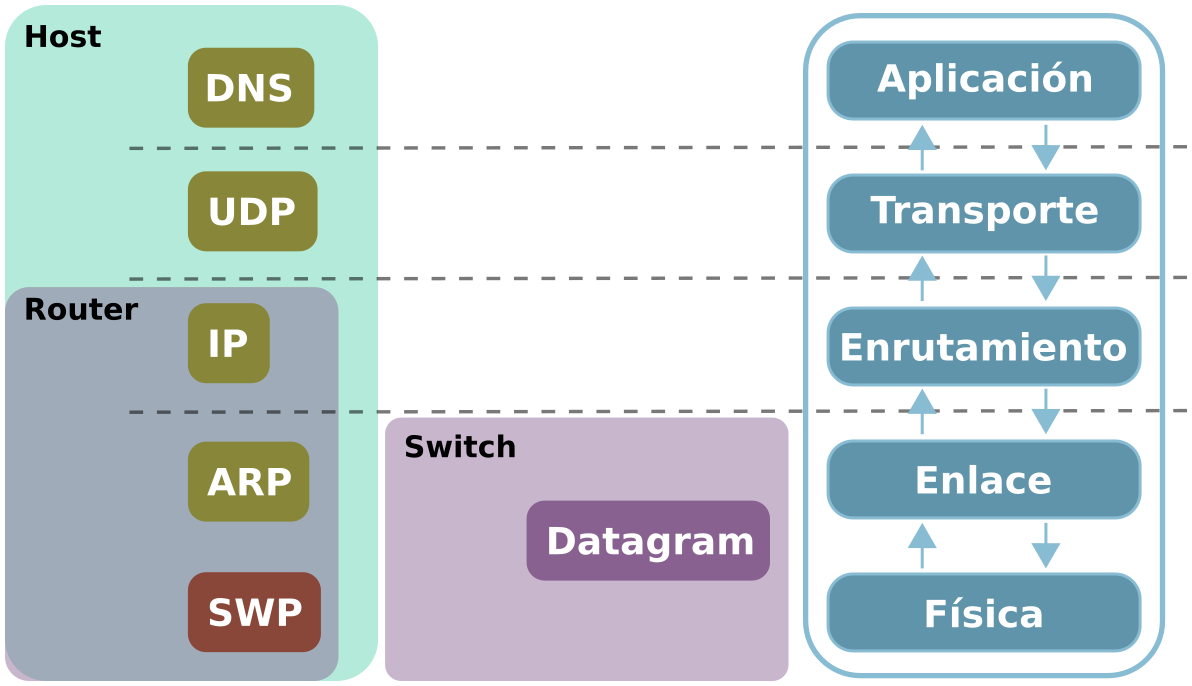
\includegraphics[width = 0.8\textwidth]{img/png/protocols.png}
    \caption{Protocolos implementados separados por capas y dispositivos que los utilizan.}
    \label{figure: protocolos}
\end{figure}
	
\subsection{DNS}
\textit{DNS} (\textit{Domain Name System}) es un sistema de indexación mediante el cual se puede transformar un nombre de dominio en una dirección \textit{IP} del host correspondiente. Este sistema es muy utilizado ya que para los humanos es muy difícil recordar direcciones en formato \textit{IP} pero no en formato \textit{Domian Name}. Asi como el sistema de indexación de una guia telefónica indexa por apellido y nombre para conseguir el número de teléfono de las persona, cuando se cuenta con un nombre de dominio se debe utilizar \textit{DNS} para conseguir la direccion \textit{IP} del host. Este sistema pertenece a la capa de aplicación y es utilizada por diversas aplicaciones para facilitar la comunicación con aplicaciones remotas. Ejemplos de esto son los browsers donde una persona escribe el nombre de dominio de un servidor y \textit{DNS} lo transforma en \textit{IP} para poder acceder al mismo donde se encuentra alojada la plataforma web. 

\subsubsection{Estructuras de datos correspondientes}
La estructura de datos utilizada para el sistema de \textit{DNS} es dns::Packet y cuenta con los siguientes campos:
\begin{itemize}
\item \textbf{header: } Es de tipo dns::Header, cuanta entre otras cosas, con toda la información necesaria para saber cuantos dns::ResourceRecord hay en cada una de los siguientes campos. La Figura \ref{figure: dns header} muestra esta estructura de datos.
\item \textbf{questions: } Una lista de dns::ResourceRecord que almacena el nombre de dominio del cual se desea obtener el \textit{IP} asociado.
\item \textbf{answers: } Una lista de dns::ResourceRecord que almacena la respuesta obtenida mediante \textit{DNS}.
\item \textbf{authoritatives: } Una lista de dns::ResourceRecord que almacena la dirección \textit{IP} de servidores \textit{DNS} mediante los cuales se puede obtener la dirección pedida.
\item \textbf{aditionals: } Una lista de dns::ResourceRecord donde se guarda la dirección ip del host que mandó el request. De esta forma no necesita pedirle a la capa \textit{UDP} por el ip que mandó el \textit{request}.
\end{itemize}

\begin{figure}[!htb]
    \centering
    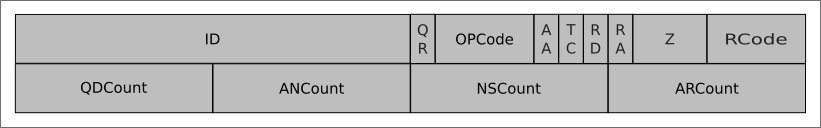
\includegraphics[width = 0.8\textwidth]{img/png/dns-header.png}
    \caption{Estructura del tipo de datos dns::Header alineada a 4 bytes.}
    \label{figure: dns header}
\end{figure}

La Figura \ref{figure: dns header} muestra la estructura del header de un paquete dns, en el mismo se ven los campos \textbf{\textit{QDCount}}, \textbf{\textit{ANCount}}, \textbf{\textit{NSCount}} y \textbf{\textit{ARCount}} que indican la cantidad de dns::ResourceRecords en cada una de las secciones \textbf{\textit{questions}}, \textbf{\textit{answers}}, \textbf{\textit{authoritatives}}, \textbf{\textit{aditionals}} respectivamente. No todos los campos son utilizados en la implementación realizada en este trabajo, la utilización de los mismos será explicada a continuación junto con la explicación del funcionamiento del protocolo. Información detallada sobre cada campo del header puede ser encontrada en \cite{dnsheader}\\

dns::ResourceRecord es la estructura de datos encargada de guardar información de pares de pregunta/respuesta. Si bien la pregunta es siempre de tipo dns::DomainName, la respuesta puede no siempre ser de tipo \textit{IP}, en algunos casos como en los renombres de dominios, o en las consultas no recursivas, la respuesta puede ser  de tipo dns::DomainName.\\

Los campos de la estructura dns::ResourceRecord son los siguientes:

\begin{itemize}
\item \textbf{name: } Es de tipo dns::DomainName y guarda el nombre de dominio del cual se quiere conocer su \textit{IP}.
\item \textbf{QType: } Indica el tipo de respuesta; A = 1 representa respuestas de servidores autoritativos y son de tipo \textit{IP}, NS = 2 representa redirecciones a un servidor autoritativo para una determinada zona y son de tipo dns::DomainName.
\item \textbf{Avalue: } Si la respuesta es de tipo A, este campo guarda el \textit{IP} correspondiente a la respuesta.
\item \textbf{NSValue: } Si la respuesta es de tipo NS, este campo guarda el dns::DomainName correspondiente a la respuesta.
\item \textbf{QClass: } Este campo indica el protocolo a utilizar; En este trabajo y en la mayoría de los casos, este campo se mantiene siempre con el valor IN = 1 = Internet protocol.
\item \textbf{TTL: } Es el tiempo de vida (generalmente en segundos) utilizado para saber cuanto tiempo se puede mantener un recurso obtenido por un pedido \textit{DNS} en la memoria cache antes de considerar que es invalido y eliminarlo.
\end{itemize}

Por último dns::DomainName es una estructura que sirve para guardar nombres de dominios como por ejemplo ``\textit{network.devs.com}''. El mismo cuenta con métodos que permiten leer, escribir, imprimir y trabajar fácilmente con la jerarquía de zonas de los mismos. Por ejemplo, para saber si un nombre de dominio pertenece a la zona de otro nombre de dominio, Se puede hacer lo siguiente: \\

dns::DomainName(``\textit{com}'').isZoneFor(``\textit{network.devs.com}'').
\subsubsection{Funcionamiento del protocolo}

\paragraph{cliente}
El protocolo implementado en este trabajo para el cliente es muy simple, las consultas comienzan con un dns::Packet que tiene un solo RR (dns::ResourceRecord) en la sección \textit{questions} que contiene el nombre de dominio del cual se desea saber el \textit{IP}. El Protocolo comienza buscando el nombre de dominio del RR en el cache y si lo encuentra devuelve el \textit{IP} asociado y terminó la consulta. En caso de que no lo encuentre los siguientes pasos son realizados:

\begin{enumerate}
\item Le asigna un nuevo ID al dns::Header del dns::Packet de la consulta.
\item Le asigna el valor QR = 1 para indicar que es una query y no un answer.
\item Le asigna el valor RD = 1 para indicar que desea que la consulta se resuelva de forma recursiva, si el servidor no es recursivo este campo será ignorado y enviara una redirección a otro servidor.
\item Guarda el paquete en una tabla de consultas realizadas localmente (i.e. consultas realizadas por el host local).
\item Agrega un RR A la sección \textit{aditionals} que contiene el IP local para que el servidor sepa a quien devolver la respuesta.
\item Envía el paquete al servidor local para que el mismo resuelva el pedido.
\end{enumerate}

\paragraph{Servidor recursivo}
Cuando un servidor recursivo recibe un dns::Packet con el campo QR = 1, el mismo intenta primero resolver la consulta buscando en la tabla de nombres de dominios para los cuales el es autoritativo. envía la respuesta realizando los siguientes pasos:

\begin{enumerate}
\item Al paquete entrante le cambia el campo QR = 0 para indicar que es una respuesta.
\item Asigna el valor AA = 1 para indicar que la respuesta proviene de un servidor autoritativo para ese nombre de dominio.
\item Le agrega un RR en la sección \textit{answers} con \textit{Qtype} = A, con el nombre de dominio de la consulta y en \textit{AValue} el IP correspondiente al nombre de dominio.
\item Envía el dns::Packet de retorno al servidor que envió el \textit{request}, el IP del mismo se encuentra en el RR de la sección \textit{aditional}.
\end{enumerate}

En caso de no encontrar la respuesta en su lista personal, si el paquete dns tiene el campo RD = 1 el servidor realiza los siguientes pasos con la finalidad de conseguir la respuesta mediante otros servidores de forma recursiva:

\begin{enumerate}
\item Guarda el paquete en una tabla de consultas realizadas remotamente (i.e. consultas realizadas por un \textit{host} remoto que llegó a través de paquetes dns).
\item Cambia el RR de la sección \textit{aditionals} para asignarle el \textit{IP} local para que el servidor al cual reenvíe la consulta sepa como enviarle la respuesta.
\item Envía el paquete al servidor TLD que conoce.
\end{enumerate}

Una vez reenviada la consulta se queda a la espera de una respuesta de del servidor. Si el servidor es autoritativo para ese nombre de dominio ó es un servidor recursivo, le enviará una respuesta final con el \textit{IP} correspondiente que será reenviado al \textit{host} del cual llegó la consulta. Si el servidor no es ni autoritativo para la consulta ni recursivo, entonces va a devolver una redirección a un servidor autoritativo para esa zona, cuando esto ocurre, en el paquete dns de respuesta vienen dos RRs, uno en la sección \textit{answers} de tipo NS que contiene el nombre de dominio de dicho servidor y otro en la sección \textit{authoritatives} de tipo A con el \textit{IP} de dicho servidor. En este caso el paquete es reenviado a dicho servidor con la esperanza de que esté resuelva la consulta o vuelva a enviar una redirección. \\

\textbf{Note:} El \textit{IP} de dicho \textit{host} está en el paquete dns que se guardó anteriormente, y la forma de recuperarlo es utilizando el ID de la consulta que se mantiene igual durante todo el proceso. \\

\textbf{Note:} En caso de que el servidor envíe un paquete dns de error, el mismo es reenviado al \textit{host} que realizo la consulta y el protocolo falló. Esto puede ocurrir porque no se conoce de ningún servidor autoritativo para la zona del nombre de dominio consultado. \\

\textbf{Note:} El paquete enviado como respuesta final es un paquete que llega desde un servidor al cual se le realizó la consulta, y por ende el campo AA que indica si la respuesta es autoritativa o no, depende de dicho servidor. \\

En caso de que que el campo RD esté en 0, el servidor se comporta como un servidor iterativo \\

\paragraph{Servidor iterativo}

Cuando una consulta llega a un servidor iterativo, en caso de ser autoritativo para la consulta, envía el paquete previamente transformado en respuesta con el \textit{IP} correspondiente a la consulta asignando AA = 1 y termina. En caso de no ser autoritativo, el servidor busca en la tabla de \textit{DN servers} un servidor que sea autoritativo para la zona del nombre de dominio consultado, en caso de haber más de uno, elige el servidor más puntual y lo envía como respuesta de redirección. Para esto realiza los siguientes pasos modificando el paquete de la consulta para mantener el ID correcto.

\begin{enumerate}
\item Agrega un RR de tipo NS en la sección \textit{answers} donde \textit{name} contiene el nombre de dominio para el cual el servidor es responsable de todos sus sub-dominios (i.e. es responsable de esa zona), y en \textit{NSValue} el nombre de dominio del servidor.
\item Agrega un RR de tipo A en la sección \textit{authoritatives} donde \textit{name} es igual al campo \textit{NSValue} del RR mencionado en el punto anterior y en el campo \textit{AValue} el \textit{IP} de dicho servidor.
\item Asigna AA = 0 para marcar que el no es autoritativo para dicha consulta.
\item Utiliza el RR de la sección \textit{aditionals} para enviar el paquete con la respuesta al host que realizó la consulta.
\end{enumerate}

\textbf{note: } un servidor $s1$ es más puntual para una zona que otro servidor $s2$ si y solo si $s1$ pertenece a la zona de $s2$, por ejemplo ``devs.com'' es más puntual que ``com'' ya que ``devs.com'' pertenece a la zona ``com'', con lo cual, si hay una consulta ``algo.devs.com'' el servidor que tiene la respuesta final es ``devs.com'' y no ``com'' quien va a devolver una redirección a ``devs.com''.

\subsection{UDP}

\subsubsection{Estructuras de datos correspondiente a UDP}

El protocolo UDP implementado cuenta con los siguientes tipos de datos, los cuales tienen documentación en formato Doxigen en el códifo y que se encuentra adjunta en el apéndice de este documento:

\begin{itemize}
\item udp::Segment: Representa un segmento de datos para ser enviado por la red, el mismo cuenta con pseudoheader, header y payload como se muestra en la Figura \ref{figure: udp segment}.
\item udp::Control: Es la estructura de datos utilizada para la comunicación con la capa de aplicación, en la misma se especifica que comando envía la aplicación a la capa UDP. Toda la información a enviar llega al protocolo UDP a través de esta estructura.
\end{itemize}

\begin{figure}[!htb]
    \centering
    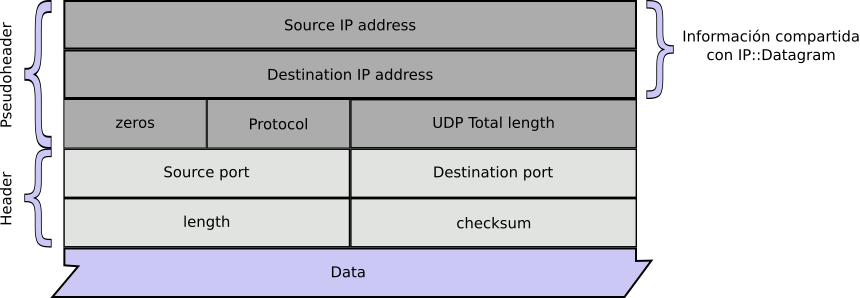
\includegraphics[width = 0.7\textwidth]{img/png/UDP-Segment.png}
    \caption{Estructura del tipo de datos udp::Segment alineada a 4 bytes.}
    \label{figure: udp segment}
\end{figure}

\subsubsection{Comportamiento del protocolo}

El protocolo UDP no cuenta con ningún sistema de detección de fallas en la entrega de los mensajes ya que el mismo está pensado para funcionar de forma que optimice la velocidad de entrega, para esto se basa en un mecanismo de mejor esfuerzo. Esto lo convierte en un buen protocolo cuando la eficiencia es un atributo clave. Por otro lado, dado que no controla que los mensajes lleguen o no a su destino, es necesario contar con otro mecanismo que detecte mensajes faltantes (aquellos que no llegaron a destino) o de lo contrario, debe permitirse la perdida de los mismos. Si bien no se realiza ningún esfuerzo por detectar si el mensaje llega o no a destino, UDP implementa checksum para detectar errores en la codificación del header del segmento, esto es implementado con la finalidad de no entregar mensajes a destinatarios incorrectos. Cuando un error es detectado en el header, el segment es directamente descartado\footnote{No se comprueba que el payload contenga errores en su codificación, por lo que el dato en si, podría llegar a destino con errores y nunca serían detectados por UDP.}.\\

UDP funciona con sockets, los sockets son una combinación de IP y puerto que permiten enviar y entregar los mensajes a la aplicación correspondiente dentro del host de destino. De esta forma, para que un mensaje sea correctamente entregado, el host destino tiene que tener una aplicación que esté escuchando por el puerto al cual fue enviado el mensaje, si este no es el caso, el mensaje es simplemente descartado. Los sockets también cumplen el roll de evitar colisiones entre las aplicaciones ya que las mismas no pueden conectarse a un puerto mediante un socket si el puerto ya está siendo utilizado por otra aplicación, ya sea para enviar o recibir mensajes. La Figura \ref{figure: UPD state machine} muestra la máquina de estados del protocolo UDP implementado en este trabajo. \\

\begin{figure}[t]
    \centering
    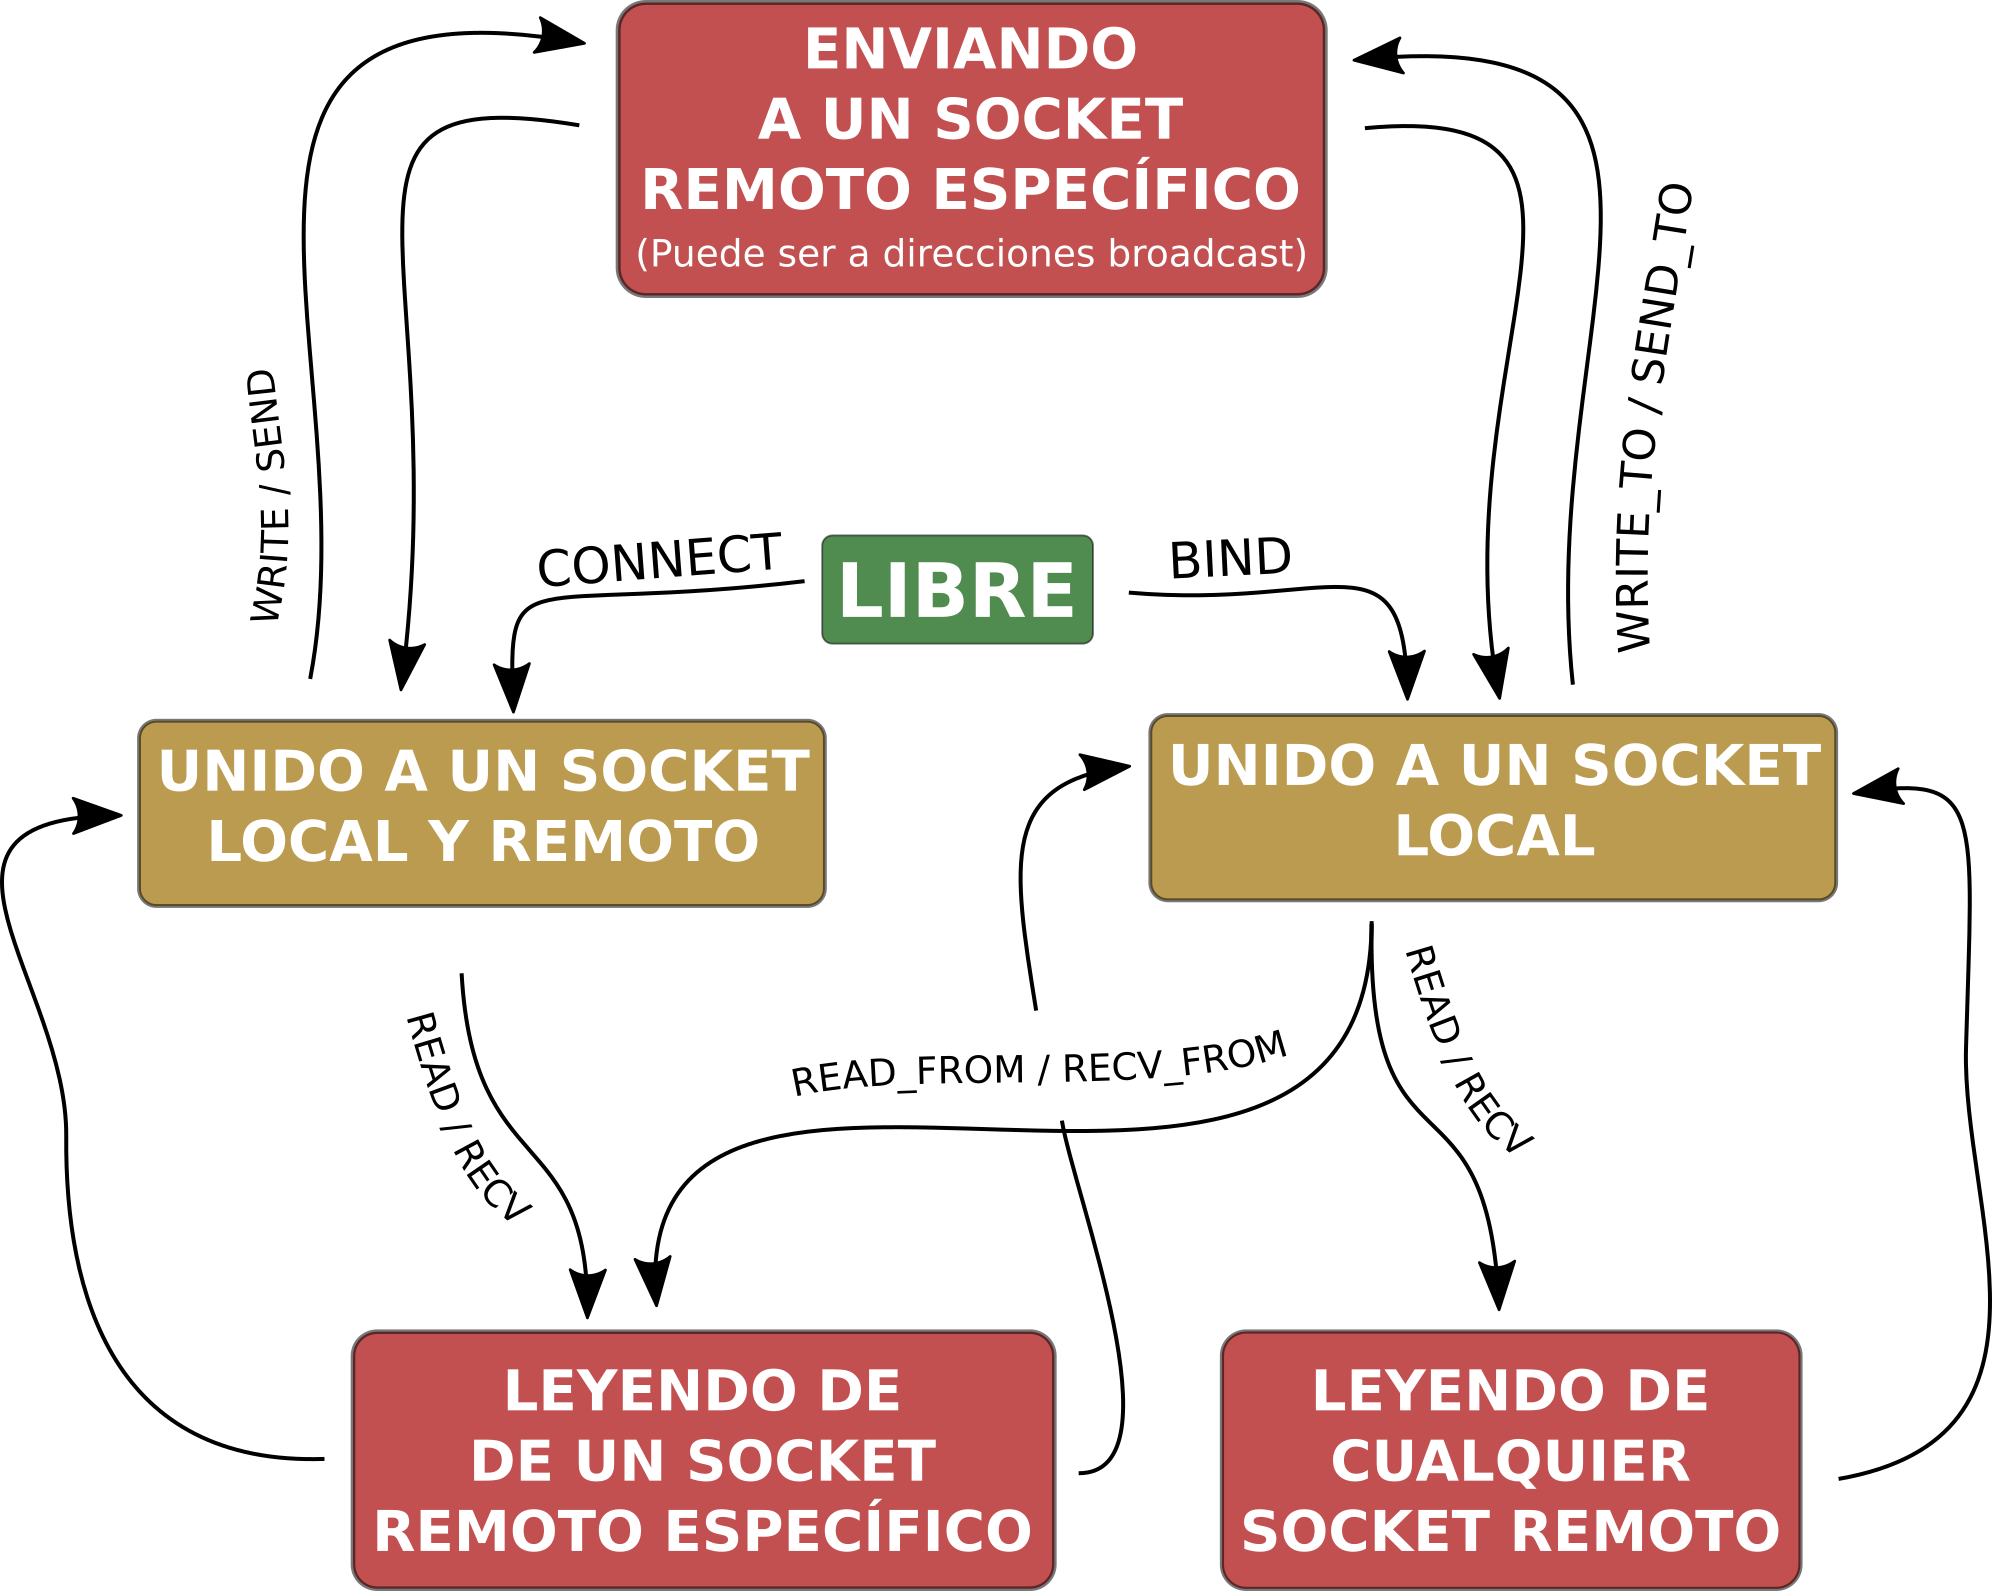
\includegraphics[width = 0.7\textwidth]{img/png/UDP-state-machine.png}
    \caption{Máquina de estados del protocolo UDP para un socket determinado. Por prolijidad, el comando \textit{CLOSE} no aparece, el mismo corta cualquier estado y vuelve automáticamente a \textit{LIBRE}.}
    \label{figure: UPD state machine}
\end{figure}

\newpage
 
En el modelo implementado, los mensajes de Control contienen un campo \textit{request} que indica que operación se desea efectuar (connect, bind, read, etc) también es necesario enviar el IP y puerto del socket y el id de la aplicación, esta información es siempre requerida, ya sea para crear un nuevo socket atado a la aplicación del id o para corroborar que el socket existe y que corresponde a la aplicación que envía el mensaje de control. Dependiendo de la operación, es preciso completar correctamente los campos restantes. A continuación se explica cada operación y que campos requiere cada una: \\

\begin{itemize}
\item \textbf{CONNECT}: \textit{remote\_ip}, \textit{remote\_port}. De está forma UDP sabe que cada vez que esta aplicación envíe o reciba un paquete, el mismo será para o desde el socket con IP \textit{remote\_ip} y puerto \textit{remote\_port}. Esta operación falla si el socket ya existe.
\item \textbf{BIND:} Esto permite a la aplicación enviar paquetes a distintos destinos, especificando siempre el socket del destino mediante los comandos WRITE\_TO y SEND\_TO y recibir mensajes de distintos orígenes mediante los comandos READ\_FROM, RECV\_FROM, REC o READ. Esta aplicación falla si el soquet ya existe.
\item \textbf{READ\_FROM / RECV\_FROM:} \textit{remote\_ip}, \textit{remote\_port}, estos campos son utilizados para saber que mensajes entrantes deben que ser aceptados y cuales no. Cuando este comando es recibido por UDP, el socket correspondiente es marcado como ``En espera de mensajes'' y el mismo se mantiene en ese estado hasta que llega un mensaje del host remoto indicado, en ese momento el mensaje es entregado y el socket vuelve al estado anterior. Este comando solo puede ser utilizado en un socket que está en estado \textit{BOUND}, o sea, un socket que fue previamente bindeado.
\item \textbf{READ / RECV:} Es lo mismo que el item anterior pero con la diferencia de que no se especifica un socket remoto. Si el el soket local fue bindeado se aceptan todos los mensajes entrantes a este socket y si fue conectado se aceptan solo los mensajes del socket remoto indicado en el momento de la conexión.
\item \textbf{WRITE\_TO / SEND\_TO:} Lo mismo que READ\_FROM / RECV\_FROM pero para enviar mensajes, con lo cual el campo \textit{packet} debe contener el paquete a enviar.
\item \textbf{WRITE / SEND:} Lo mismo que READ / RECV pero para enviar mensajes, con lo cual el campo \textit{packet} debe contener el paquete a enviar.
\item \textbf{CLOSE:} Esta operación remueve el socket, dejando el IP y puerto libres para futuras aplicaciones que quieran conectarse o bindearse al mismo.
\end{itemize}

Cada vez que el protocolo UDP quiere enviar un paquete, crea un nuevo udp::Segment, asigna el paquete en el campo \textit{payload} en formato \textit{char *} de no más de $512$ bytes de tamaño, completa los campos correspondientes del header y pseudoheader, calcula el checksum utilizando el header ya completado, guarda el valor obtenido en el campo \textit{checksum} y envía el mensaje a la capa inferior por el canal de datos encolando el mismo en la cola \textit{lower\_layer\_data\_out}. \\

Cada vez que el protocolo UDP recibe un mensaje de la capa inferior se realizan un par de chequeos, en caso de que el mensaje pase los controles, el \textit{payload} del segmento recibido es entregado a la aplicación correspondiente, en caso contrario el segmento es descartado. Un segmento pasa los chequeos si se cumplen las siguientes condiciones:

\begin{itemize}
\item El campo \textit{checksum} debe coincidir con el calculo de checksum que realiza nuevamente el protocolo sobre el header del segmento recibido.
\item El socket destino del segmento debe ser un socket local existente.
\item El socket local debe estar en un estado de ``En espera de mensajes''.
\item El socket local debe estar esperando mensajes del socket remoto o esperando mensajes de cualquiero socket remoto.
\end{itemize}

La estructura de datos \textit{Socket} es utilizada para manipular esta combinaciones de ip-puerto, la misma cuenta con los siguientes campos.

\begin{itemize}
\item \textbf{local\_port: } Es de tipo \textit{uint\_16} y representa el puerto del host local al cual se conecta o bindea el socket.
\item \textbf{remote\_port: } Es de tipo \textit{uint\_16} y representa el puerto del host remoto al cual se desea enviar y/o recibir datos. Este campo es opcional, no siempre se especifica un host remoto, por ejemplo, cuando se desea leer datos de cualquier host remoto, este campo no debe especificarse.
\item \textbf{local\_ip: } Es de tipo \textit{IPv4}\footnote{El tipo de datos \textit{IPv4} está documentado en formato Doxigen en el código} y representa el ip del host local al cual se conecta o bindea el socket.
\item \textbf{remote\_ip: } Es de tipo \textit{IPv4} y representa el ip del host remoto al cual se desea enviar y/o recibir datos. Este campo es opcional, no siempre se especifica un host remoto, por ejemplo, cuando se desea leer datos de cualquier host remoto, este campo no debe especificarse.
\item \textbf{status: } Es de tipo enum e indica en que estado se encuentra el socket. Los estados son los mencionados previamente cuando se explicaron los comandos.
\end{itemize}

La Tabla \ref{table: parameters UDP} muestra los parámetros del modelo UDP en la IDE PowerDEVS.
\begin{table*}[h]
\begin{tabular}{|l|c|c|c|}
  \hline
  \textbf{Nombre} & \textbf{Tipo} & \textbf{Descripción} \\
  \hline
  Module name & String & El nombre del módulo que utiliza el logger \\
  \hline
  ip\_amount & Int & La cantidad de ip locales, generalmente este valor es 1 \\
  \hline
  ip 1 & IPv4 & La primer ip local \\
  \hline
  \vdots & \vdots & \vdots \\
  \hline
  ip n & IPv4 & La última ip local \\
  \hline
\end{tabular}
\caption{Parámetros del modelo UDP}
\label{table: parameters UDP}
\end{table*}

\subsection{IP}

El protocolo IP es el encargado del enrutamiento de los ip::Datagrams de un nodo (router, host) a otro con la finalidad de llegar al host destino. La estructura de datos ip::Datagram es la utilizada para encapsula los udp::Segments y cuenta con un campo \textit{header} de tipo ip::Header y un campo \textit{data} de tipo udp::Segment, la Figura \ref{figure: ip header} muestra la estructura del tipo de datos ip::Header.  \\

\begin{figure}[!htb]
    \centering
    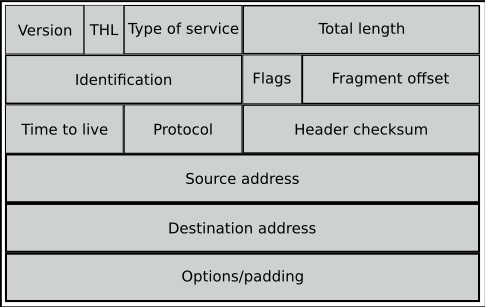
\includegraphics[width = 0.4\textwidth]{img/png/IP-datagram.png}
    \caption{Estructura del tipo de datos de ip::Header alineada a 4 bytes.}
    \label{figure: ip header}
\end{figure}

El protocolo IP implementado en este trabajo funciona con UDP y se puede dividir en dos categorías:
\begin{itemize}
\item \textbf{Enrutamiento en un host:} Los hosts son los encargados de encapsular los udp::Segments provenientes de la capa superior (UDP) dentro de ip::Datagrams y enviarlos al router o host directamente conectado al mismo dependiendo de si el IP de destino corresponde a un un host de la misma subnet o a un host en otra subnet. Si un host recibe un ip::Datagram cuyo IP destino no corresponde con ningún IP del host, el ip::Datagram no es forwardeado a nadie y es descartado, en cambio si el IP corresponde con algún IP del host, el udp::Segment del ip::Datagram recibido es desencapsulado y entregado a la capa superior.
\item \textbf{Enrutamiento en un router:} Los routers por el contrario no encapsulan udp::Segments ya que no existe capa de transporte en un router, los mismos se encargan de forwardear ip::Datagrams que llegan.
\end{itemize}

Si bien hay diferencia entre los hosts y los routers, el proceso de forwardear ip::Datagrams es el mismo para ambos, este proceso consiste en buscar el mejor \textit{nexthope} dentro de la ``routing table'' y enviar el ip::Datagram al mismo con la esperanza de que este sepa como entregar el mensaje al destino. \\

En este trabajo no se implementaron clases de direcciones IP A, B y C, por el contrario se implementó el mecanismo de \textit{subneting} mediante el uso de \textit{netmasks}, esto significa que se utiliza una máscara que indica cuantos bits de la izquierda del IP corresponden al network. La máscara utilizada es una dirección IP que tiene en los bits de la izquierda unos y en los bits de la derecha ceros, la cantidad de unos de la máscara determinan cuantos bits del IP deben ser considerados como network. \\

La routing table contiene los siguientes campos:
\begin{itemize}
\item \textbf{Network:} IP del network asociado a esta entrada.
\item \textbf{Netmask:} Máscara utilizada para saber que parte del IP network debe ser comparada con el IP destino para determinar si el IP destino corresponde a la misma red a la cual se puede llegar mediante este netxhope.
\item \textbf{Nexthope:} IP del nodo al cual hay que enviarle el ip::Datagram de forma que el mismo sepa como entregar el ip::Datagram. El nexthope debe estar directamente conectado con el nodo actual. El mismo puede ser un host, en este caso, el destino es directamente alcanzable y el mensaje es enviado al mismo.
\item \textbf{Metric:} Una métrica de a que distancia (en termino de nodos intermedios) se encuentra el destino del router o host actual.
\item \textbf{Description:} Una descripción que ayude a comprender el rol del nexthope. Esto puede ser el nombre del mismo.
\end{itemize}

Para determinar cual \textit{nexthope} es el mejor se utiliza el siguiente criterio: Se elige aquel nexthope con prefijo de network más pequeño, si hay más de uno con menor prefijo, se elige aquel con menor métrica, o sea, aquel para el cual se espera que el camino sea menor, si sigue siendo necesario desempatar, se elige el primero de la tabla de arriba para abajo. \\

Un dispositivo puede tener más de una interfaz, cada interfaz está conectada con una network particular y el \textit{nexthope} elegido pertenece a alguna de esas networks, para saber por que interfaz enviar el ip::Datagram se utiliza la \textit{forwarding table} la cual indica para cada \textit{nexthope} su interfaz asociada dependiendo de en que network se encuentre el \textit{nexthope}. \\

Dado que en este trabajo no se implementó ningún algoritmo dinámico para completar las \textit{routing table} y \textit{forwarding table}, si las mismas no son correctamente inicializadas a mano, puede suceder que un paquete nunca llegue a destino o que el mismo se quede dando vueltas en círculos. Para evitar que se generen ciclos infinitos que ocasionarían una gran congestión de la red, se utiliza el campo \textit{TTL} (Time To Live) el cual arranca con el valor $255$ cuando el host envía el paquete al primer \textit{nexthope} y es decrementado en uno cada vez que pasa por un nuevo router, de esta forma, cuando el \textit{TTL} llega a $0$ el ip::Datagram es descartado en vez de ser forwardeado. Este tipo de problemas puede suceder también cuando las \textit{routing tables} son completadas dinámicamente. \\

Para poder enviar un ip::Datagram al nexthope o al host en cuestión, el protocolo IP le manda un mensaje de control a la capa de linkeo para pedirle que prepare la MAC address asociada al IP del \textit{nexthope}, una vez que recibe el mensaje de la capa de linkeo confirmando que dicha MAC address está cacheada, el protocolo IP pasa el ip::Datagram a la capa de linkeo para que el mismo lo envíe. El mensaje de confirmación de que la \textit{MAC address} existe no asegura que el mensaje sea enviado, en caso de que un error acontezca en el protocolo ARP, el mismo se lo comunica a IP que se queda esperando una nueva confirmación del protocolo ARP comunicando que el envío puede ser realizado. \\

Los parámetros del modelo IP en la IDE de PowerDEVS son los que muestra la Tabla \ref{table: parameters ip}

\begin{table*}[h]
\begin{tabular}{|l|c|c|c|}
  \hline
  \textbf{Nombre} & \textbf{Tipo} & \textbf{Descripción} \\
  \hline
  Module name & String & El nombre del módulo que utiliza el logger \\
  \hline
  ip\_amount & Int & La cantidad de ip locales, generalmente este valor es 1 \\
  \hline
  ip 1 & IPv4 & La primer ip del host \\
  \hline
  \vdots & \vdots & \vdots \\
  \hline
  ip n & IPv4 & La última ip del host \\
  \hline
  file\_path\_rt & String & Path al archivo que contiene las entradas de la routing table \\
  \hline
  file\_path\_ft & String & Path al archivo que contiene las entradas de la fowarding table \\
  \hline
\end{tabular}
\caption{Parámetros del modelo IP}
\label{table: parameters ip}
\end{table*}

\subsection{ARP}

Si bien los IPs cuentan con una estructura jerárquica que permite describir la topología de la red y de esa forma agrupar a los hosts por networks, los mismos son asignados dinámicamente dependiendo de en donde está conectado el host. Por el contrario, las \textit{MAC addresses} son fijas, y cada dispositivo de red viene con una \textit{MAC address} de fábrica, la misma se supone que es única. Para poder enviar datos de un dispositivo a otro, es necesario primero conseguir su \textit{MAC address}, el protocolo ARP (\textit{Address Resolution Protocol}) es el encargado en este modelo para realizar este trabajo. \\

Los ip::Datagram que deben ser enviados entre dos nodos adyacentes de la red son encapsulados dentro de un link::Frame, el cual cuenta con la estructura mostrada en la Figura \ref{figure: frame structure}. \\

\begin{figure}[!htb]
    \centering
    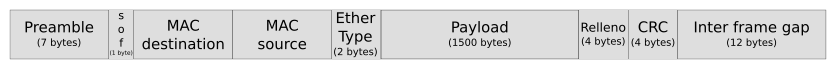
\includegraphics[width = 0.9\textwidth]{img/png/l2-frame.png}
    \caption{Estructura de datos de un link::Frame.}
    \label{figure: frame structure}
\end{figure}

El campo payload es el que contiene al ip::Datagram, el mismo admite un tamaño máximo de $1500$ bytes, por lo cual todos los paquetes enviados en este modelo deben tener un tamaño menor a $1500$ bytes \footnote{En este trabajo no está implementado el mecanismo de fragmentación}. El campo \textit{MAC\_destination} es el que contiene el \textit{MAC address} del dispositivo de destino al cual se desea enviar el frame.\\

El protocolo ARP cuenta con una \textit{ARP table}, la cual tiene las siguientes columnas:

\begin{itemize}
\item \textbf{ip:} El IP del dispositivo al cual se debe enviar el link::Frame, este IP es el que utiliza la capa IP.
\item \textbf{mac:} La \textit{MAC address} del dispositivo al cual se debe enviar el link::Frame.
\item \textbf{timeout:} Es el periodo de tiempo de validez que tiene el dato. Cada vez que se agrega una fila a la \textit{ARP table}, al mismo se le asigna un \textit{timeout}, y cuando el mismo se acaba, la fila es eliminada de la tabla.
\end{itemize}

Cada vez que el protocolo IP envía un pedido para enviar un ip::Datagram, el protocolo ARP busca el IP en la \textit{ARP Table}, si hay una entrada con ese IP, ARP manda un mensaje de control a la capa IP comunicando que el envío puede ser efectuado, si por el contrario, no hay una entrada con ese IP, ARP envía un link::arp::Packet con un pedido de \textit{MAC} a todos los dispositivos de la red directamente conectados con el. Todo dispositivo que recibe un link::arp::Packet con pedido de \textit{MAC} cuya dirección IP corresponda con la requerida, enviará una respuesta con su \textit{MAC address}, luego, el dispositivo que envió el pedido, al recibir la respuesta agrega la nueva entrada a la \textit{ARP table}. Una vez que se obtuvo la \textit{MAC address}, ARP envía el mensaje de control a la capa IP comunicando que el envío puede ser efectuado. Si ningún dispositivo de la red matchea con el IP solicitado, entonces el ip::Datagram nunca será enviado pues el protocolo ARP se quedará hasta el infinito esperando la respuesta de la red, esto no implica que el protocolo quede bloqueado y otros pedidos podrían ser procesados.\\

Podría suceder que durante el tiempo que transcurre entre que ARP envía el mensaje a IP comunicándole que el envío puede realizarse y que el protocolo IP manda el ip::Datagram para ser enviado, el \textit{timeout} de la \textit{MAC address} requerida se cumpla y la misma sea eliminada de la tabla. Si este es el caso, se envía un mensaje al protocolo IP de falla en el envío del ip::Datagram y se vuelve a mandar un link::arp::Packet para volver a obtener el \textit{MAC address}. La figura \ref{figure: ARP IP comunication flow} muestra la comunicación entre ARP y IP para la obtención de la \textit{MAC address} y la Figura \ref{figure: arp packet} muestra la estructura de un link::arp::Packet.\\

\begin{figure}[!htb]
    \centering
    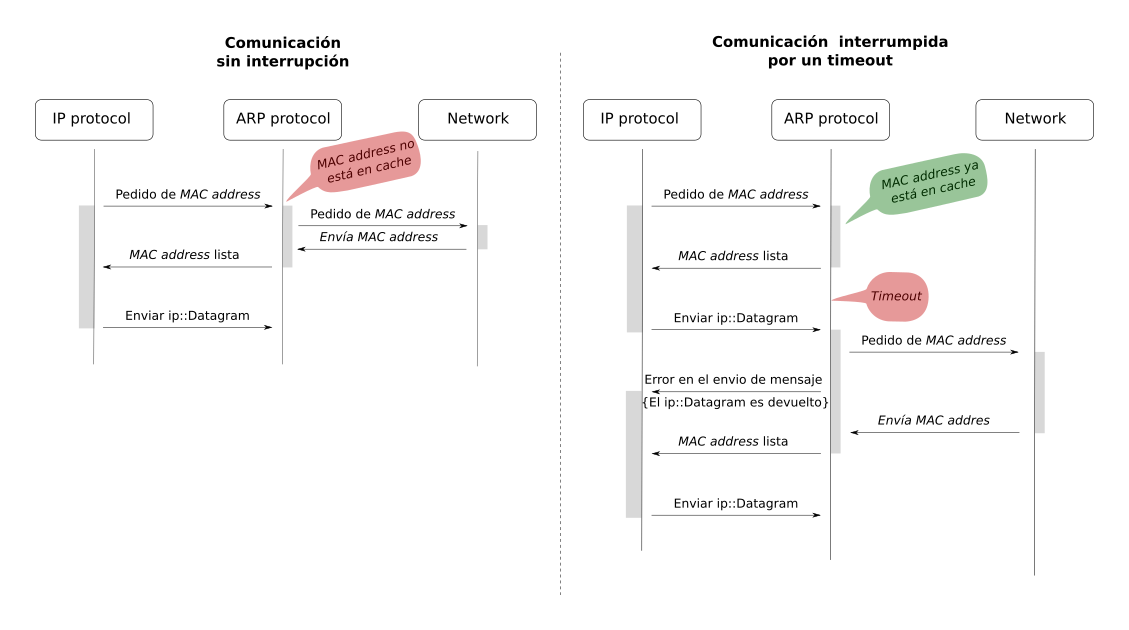
\includegraphics[width = 0.8\textwidth]{img/png/ip-arp-comunication.png}
    \caption{Flujo de comunicación entre los protocolos IP y ARP para enviar un ip::Datagram.}
    \label{figure: ARP IP comunication flow}
\end{figure}

\begin{figure}[!htb]
    \centering
    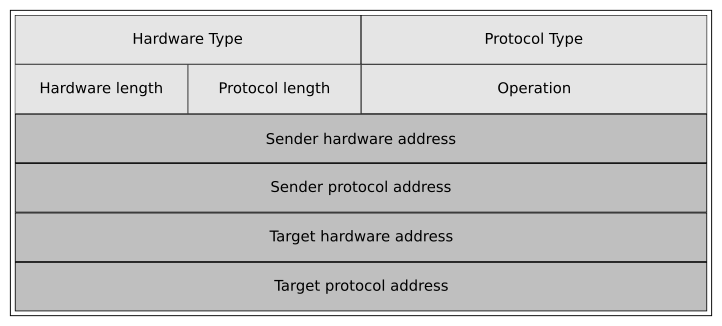
\includegraphics[width = 0.6\textwidth]{img/png/arp-packet.png}
    \caption{Estructura de datos de un link::arp::Packet alineada a 4 bytes. \textbf{Nota:} las direcciones de hardware (\textit{MAC addresses}) son de 6 bytes y no de 4, esto no se muestra en la figura para mantener el orden de los campos.}
    \label{figure: arp packet}
\end{figure}


Un dispositivo puede tener varias interfaces y cada interfaz es un modelo \textit{Link} que implenta ARP y SWL. Este es el caso de los routers que cuentan con una interfaz por cada network al que están conectados. Cada interfaz cuanta con un IP y con una \textit{MAC address} y los pedidos de \textit{MAC address} que llegan a la interfaz son respondidos por el protocolo ARP dentro de la interfaz sin llegar a la capa de enrutamiento. De esta forma, un router puede ser accedido por los dispositivos de una red solo si ellos conocen el IP de la interfaz que está conectada a dicha red, en caso de que llegue un pedido de \textit{MAC address} para un IP de otra interfaz, el mismo es ignorado ya que las interfaces son independientes entre si. \\

Tanto \textit{ARP} como \textit{SWP} (explicado más adelante) son protocolos de nivel 2 y es por eso que se encuentran ambos implementados dentro del modelo \textit{link}. La tabla \ref{table: parameters link} muestra los parámetros del modelo de \textit{link} en la IDE PowerDEVS. 

\begin{table*}[h]
\begin{tabular}{|l|c|c|c|}
  \hline
  \textbf{Nombre} & \textbf{Tipo} & \textbf{Descripción} \\
  \hline
  Module name & String & El nombre del módulo que utiliza el logger \\
  \hline
  Mac & MAC & la mac address de la interfaz \\
  \hline
  ip & IPv4 & La ip de la interfaz \\
  \hline
  interface & Int & El número de la interfaz \\
  \hline
\end{tabular}
\caption{Parametros del modelo Link}
\label{table: parameters link}
\end{table*}

\subsection{Datagrams}
El protocolo Datagrams es utilizado por los switches para forwardear mensajes. \\

En el modelo implementado, el envío de frames sucede mediante cables ethernet, y para evitar colisiones, un dispositivo puede estar conectado a muchos otros mediante el uso de switches. Aunque en la realidad los switches evitan gran parte de las colisiones, los mismos no evitan todas, ya que siguen existiendo las colisiones generadas entre los frames que se envían de cada punta del cable. Este tipo de colisiones no están consideradas y el modelo implementado se abstrae de ellas, dejándolo como posible trabajo futuro. \\

El trabajo principal de un switch es el de forwardear frames que llegan por un puerto de entrada a través de un puerto de salida de forma de que el frame llegue al destinatario. Para realizar esta tarea, el protocolo implementado es \textit{Datagrams} explicado en el libro de cabecera de la cátedra \cite[p.~172]{peterson2011computer}. El mismo tiene un funcionamiento muy sencillo, utiliza una \textit{forwarding table} que contiene las siguientes columnas: \\

\begin{itemize}
\item \textbf{mac: } La \textit{MAC address} del destinatario.
\item \textbf{interface: } La interfaz o puerto por donde debe forwardear el frame para llegar al destinatario.
\end{itemize}

Cada vez que un nuevo frame llega a un switch, el mismo busca la \textit{MAC address} del destinatario en la \textit{forwarding table} y envía el frame por el puerto correspondiente a esa \textit{MAC address}. Si dicha \textit{MAC address} no está en la \textit{forwarding table}, el frame es descartado y se logea un mensaje de error. \\

Nuevamente, en este trabajo no se implementó ningún algoritmo dinámico para completar las \textit{forwarding tables} de los switches y las mismas deben ser completadas a mano, si dichas tablas no están completas o están mal completadas los frames podrían nunca llegar a destino y/o quedarse dando vueltas entre los distintos switches infinitamente. \\

Tanto \textit{Datagrams} como \textit{SWP} (explicado más adelante) son protocolos de nivel 2 y es por eso que se encuentran ambos implementados dentro del modelo \textit{switch}. La Tabla \ref{table: parameters datagrams} muestra los parámetros del modelo \textit{switch}.

\begin{table*}[h]
\begin{tabular}{|l|c|c|c|}
  \hline
  \textbf{Nombre} & \textbf{Tipo} & \textbf{Descripción} \\
  \hline
  Module name & String & El nombre del módulo que utiliza el logger \\
  \hline
  Interface\_amount & Int & La cantidad de interfaces por las cuales forwardear los Frames entrantes \\
  \hline
  forwarding\_table & String & Path al archivo que contiene las entradas de la fowarding table \\
  \hline
\end{tabular}
\caption{Parámetros del modelo Switch}
\label{table: parameters datagrams}
\end{table*}

\subsection{SWP}

Este protocolo es el utilizado en la capa $2$ y el mismo se encuentra tanto en el modelo \textit{link} como en el modelo \textit{switch}, de esta forma la comunicación de todos los dispositivos a nivel $2$ es realizada mediante \textit{SWP}.\\

En este trabajo también se implementó el protocolo \textit{Sliding Window Protocol} de forma de garantizar que la comunicación entre dos dispositivos de la red se realiza sin perdida de frames y que los mismos llegan en orden, o sea, si se envía más de un paquete de un dispositivo a otro, los mismos son entregados en el mismo orden en que fueron enviados. Para no desaprovechar el ancho de banda enviando un solo frame por vez, el protocolo SWP utiliza una ventana que sirve para marcar cuantos frames pueden ser enviados en simultaneo de forma desordenada y a medida que los mismos van llegando, cuando el destinatario los ordena, la ventana se va corriendo. La Figura \ref{figure: swp timeline} ilustra la idea general del envío y recivo de mensajes mediante el protocolo SWP en una linea temporal.\\

\begin{figure}[!htb]
    \centering
    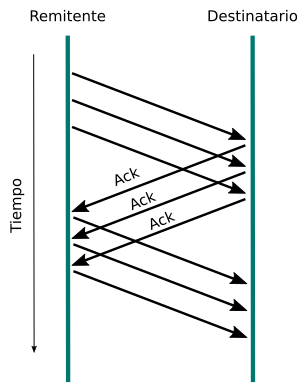
\includegraphics[width = 0.3\textwidth]{img/png/swp-timeline.png}
    \caption{Idea general de la linea temporal del protocolo SWP.}
    \label{figure: swp timeline}
\end{figure}

El protocolo SWP está separado en dos partes, el remitente y el destinatario y funcionan de la siguiente manera:

\subsubsection{Remitente:}
Cuenta con una variable \texttt{SWS} (\textit{Send Window Size}) que indica el tamaño de la ventana y una variable \texttt{LAR} \textit{Last Acknowledgment Received} que indica el último frame enviado para el cual se recibió un acknowledgment. A medida que llegan frames a enviar, se les asigna un número de secuencia (\textit{SeqNum}) correspondiente al orden de llegada y se procede a enviar todos aquellos que cumplen que \texttt{LAR} $<$ \textit{SeqNum} $\leq$ \texttt{LAR} + \texttt{SWS}. Por otro lado, cada vez que recibe un ack, mira el \textit{SeqNum} asociado al mismo y corre el inicio de la ventana (la variable \texttt{LAR}) hasta el mismo, esto automáticamente corre el final de la ventana y habilita por lo tanto nuevos frames a ser enviados. Este mecanismo funciona porque se sabe que el destinatario solo envía el ack de un frame cuando todos los frames anteriores al mismo también fueron correctamente recibidos. Cada vez que un frame es enviado, el mismo es guardado en un arreglo de frames enviados esperando que llegue un ack igual o más grande que el mismo, cuando el ack llega, el frame es descartado. Además, todo frame que es enviado se le asigna un timeout, si no se recibe un ack válido para dicho frame antes de que se termine el timeout, se considera que hubo una falla en el envío y el frame es enviado nuevamente.

\subsubsection{Destinatario:}
Cuenta con una variable \texttt{RWS} (\textit{Receive Window Size}) que indica el tamaño de la ventana de cuales \textit{SeqNum} son aceptados y con una variable \texttt{LFR} (\textit{Last Frame received}) que indica el último frame para el cual envió un acknoledgment y por ende el comienzo de la ventana. En caso de que un frame llegue y no cumpla que \texttt{LFR} $<$ \textit{SeqNum} $\leq$ \texttt{LFR} + \texttt{RWS}, el mismo es descartado. Los frames que llegan y son aceptados se guardan en un arreglo a la espera de ser entregados a la capa superior. Cada vez que un frame es aceptado, se mira cual es el frame aceptados con \textit{SewNum} más grande tal que todos los frames con \textit{SeqNum} menor a el ya fueron recibidos y se envía un ack de dicho frame. Una vez que se envió el ack de un frame, el y todos los frames anteriores son enviados a la capa superior. \\

Una cosa a tener en cuenta es que el \textit{SeqNum} está representado con un unsigned char y cuando llega al máximo número representable la secuencia vuelve a empezar de cero. Para evitar problemas con esto, es necesario asegurarse que las ventanas \texttt{SWS} y \texttt{RWS} sean lo suficientemente chicas respecto al máximo \textit{SeqNum} de forma de que cuando se llegue al mismo y se vuelva a empezar no se generen confusiones. \\

\subsection{Casos de test unitarios}

para tener una validación del comportamiento de cada uno de los módulos del modelo implementado, se realizaron distintos test de unidad, en los cuales se inventó el input de los modelos y se comparó el resultado obtenido con el esperado. De esta forma a continuación se listan todos los test unitarios implementados: \\

El único módulo que no cuenta con test de unidad, es el modelo \textit{Switch} ya que el mismo se encuentra en un modelo acoplado de dispositivo donde es el único módulo, con lo cuál, el test de integración para este caso funciona como test de unidad también. \\

Para realizar test de unidad de cada módulo por separado (un módulo representa una capa o un protocolo en específico), dado que los mismos funcionan en su totalidad mediante la interacción con el resto de los modelos y ellos no van a estar en el test (por ser de unidad y no de integración), se implementaron múltiples modelos generadores y vertederos utilizando la técnica descripta en la Sección \ref{section: I/O}. De esta forma, por cada puerto de entrada por el cual el modelo recibe un input o emite un output desde y hacia otros modelos, se mockean los inputs y se guardan en archivos los output generados por el modelo consiguiendo de esta forma emular un símulación con interacciones aunque no esten todas las partes presentes. \\

\subsubsection{Test de unidad para el módulo DNS}

En el caso del modelo DNS, el test de unidad básico implementado recibe un pedido de resolución para el dominio ``networks.devs.com'' por el puerto de entrada 0 (puerto por el cual recibe datos de la capa superior) en el tiempo virtual 15, el módulo envía un pedido recursivo a su servidor local con ip conocido 1.0.0.2 por el puerto de salida 3 y luego de que el servidor resuelve la consulta de forma recursiva, se le envia un mensaje con la respuesta en formato de paquete dns por el puerto de entrada 2 (puerto por el cual recibe datos de la capa inferior), el mismo procesa la respuesta y la reenvía por el puerto de salido 0. La Figura \ref{figure: unit test dns} muestra el modelo implementado en PowerDEVS para el test de unidad del modelo dns con sus respectivas fuentes y vertederso.

\begin{figure}[!htb]
    \centering
    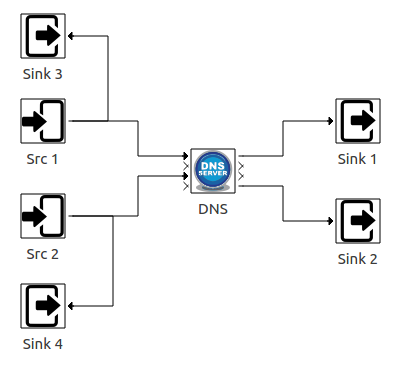
\includegraphics[width = 0.5\textwidth]{img/png/unit_tests/dns.png}
    \caption{Src 1 genera input de tipo dns::DomainName, src 2 genera input de tipo dns::Packet. Sink 1 imprime output de tipo dns::Packet y Sink 2 imprime output de tipo udp::Control, Sinks 3 y 4 imprimen el input generado por Src 1 y Src 2.}
    \label{figure: unit test dns}
\end{figure}

\newpage

A continuación se muestra el input y output del test: \\

\textbf{Input port 0 (dns::DomainName)}
\lstinputlisting[language=Bash]{../tests/dns/output/input_domain_name.output}

\textbf{Input port 2 (dns::Packet)}
\lstinputlisting[language=Bash]{../tests/dns/output/input_dns_packet.output}

\textbf{Output port 0 (dns::Packet)}
\lstinputlisting[language=Bash]{../tests/dns/output/dns_packet.output}

\newpage

\textbf{Output port 3 (udp::Control)}
\lstinputlisting[language=Bash]{../tests/dns/output/udp_control.output}

\subsubsection{Tet de unidad para el módulo UDP}

Para testear el módulo UDP se utilizó la misma lógica que para DNS. En este caso, se implementaron generadores tanto para los controles de udp que envian pedidos de conección, bindeo, etc. desde la capa superior, como para los udp::Segment que llegan desde la capa inferior. La figura \ref{figure: unit test udp} muestra el modelo implementado en PowerDEVS para el test de unidad del módulo UDP. \\

En este escenario, se simuló lo siguiente:
\begin{enumerate}
\item El módulo de capa de aplicación se conecta la aplicación con id 0 al socket local 1.0.0.1:80 y remoto 1.0.0.2:80.
\item El módulo de capa de aplicación realiza envia dos paquetes vaciós para la aplicación con id 0 utilizando el socket previamente conectado.
\item El módulo de capa de aplicación bindea la aplicación con id 1 al socket local 1.0.0.1:8080.
\item El módulo de capa de aplicación envia un paquete para la aplicación con id 1 especificando el destinatario con socket remoto 1.0.0.2:8080.
\item El módulo de capa de aplicación envia un paquete para la aplicación con id 0 por el socket local 1.0.0.1:53 inexistente, por lo que este pedido falla.
\item Una aplicación remota envía un paquete con socket remoto 1.0.0.2:80 y local 1.0.0.1:80. Si bien el socket es válido, el udp::Segment entrante falla en el checksum ya que el mismo es inválido y es descartado (esto no se ve en el output, pero se ve en el log de la simulación).
\end{enumerate}

\begin{figure}[!htb]
    \centering
    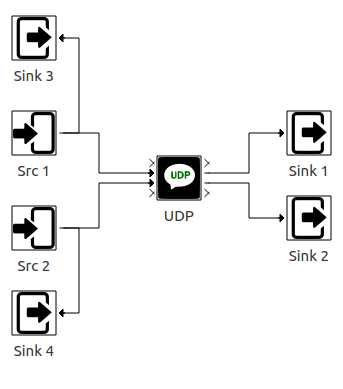
\includegraphics[width = 0.5\textwidth]{img/png/unit_tests/udp.png}
    \caption{Src 1 genera input de tipo udp::control, src 2 genera input de tipo udp::Segment. Sink 1 imprime output de tipo udp::Control, Sinks 2 imprime output de tipo udp::Segment mientras que Sink 3 y 4 imprimen el input generado por Src 1 y Src 2.}
    \label{figure: unit test udp}
\end{figure}

\newpage

A continuación se muestra el input, output y log del test: \\

\textbf{Input port 1 (udp::Control)}
\lstinputlisting[language=Bash]{../tests/udp/output/input_udp_control.output}

\textbf{Input port 2 (udp::Segment)}
\lstinputlisting[language=Bash]{../tests/udp/output/input_udp_segment.output}

\textbf{Output port 1 (udp::Control)}
\lstinputlisting[language=Bash]{../tests/udp/output/udp_control.output}

\textbf{Output port 2 (udp::Segment)}
\lstinputlisting[language=Bash]{../tests/udp/output/udp_segment.output}

\textbf{Log generado por el logger implementado}
\begin{lstlisting}
Simulation Initialized
[INFO] - [UDP Test] Connect
[INFO] - [UDP Test] SUCCESS
[INFO] - [UDP Test] Write/Send
[INFO] - [UDP Test] Write/Send
[INFO] - [UDP Test] Bind
[INFO] - [UDP Test] SUCCESS
[INFO] - [UDP Test] process Segment: 
[INFO] - [UDP Test] local_port: 80
[INFO] - [UDP Test] remote_port: 80
[INFO] - [UDP Test] local_ip: 1.0.0.1
[INFO] - [UDP Test] remote_ip: 1.0.0.2
[DEBUG] - [UDP Test] Header checksum: 0
[DEBUG] - [UDP Test] Calculated checksum: 21411
[INFO] - [UDP Test] valid checksum: False
[INFO] - [UDP Test] discarted segment.
[INFO] - [UDP Test] Write_to/Send_to
[INFO] - [UDP Test] Write/Send
[INFO] - [UDP Test] INVALID_SOCKET
Simulation Ended (0.00162 sec)
\end{lstlisting}

\subsection{Escenario implementado}

Para finalizar el modelo y a modo de test de integración, se implementó un modelo de una red y se simuló un escenario de interacción entre los \textit{host} de dicha red. El escenario implementado en este trabajo está pensado para cubrir de forma minimal los eventos relevantes en el envío de mensajes a través de la red tales como: Pasar por múltiples \textit{routers}, enviar mensajes a otro host de la misma red y enviar mensajes a un \textit{host} de una red donde es el único \textit{host}. Dado que se implementó \textit{DNS}, el escenario también busca mostrar un ejemplo interesante donde se ejecuten tanto pedidos recursivos como pedidos iterativos a los distintos servidores \textit{DNS}. Para conseguir esto, se planteo el escenario mostrado en la Figura \ref{figure: case study}, el mismo cuenta con cinco \textit{subnets} con diferentes cantidades de \textit{switches} y \textit{hosts}, las \textit{subnets} $2$ y $3$ no cuentan con dispositivos extras a los \textit{routers} a los cuales están conectadas ya que no aportaría nada nuevo. \\

\begin{figure}[!htb]
    \centering
    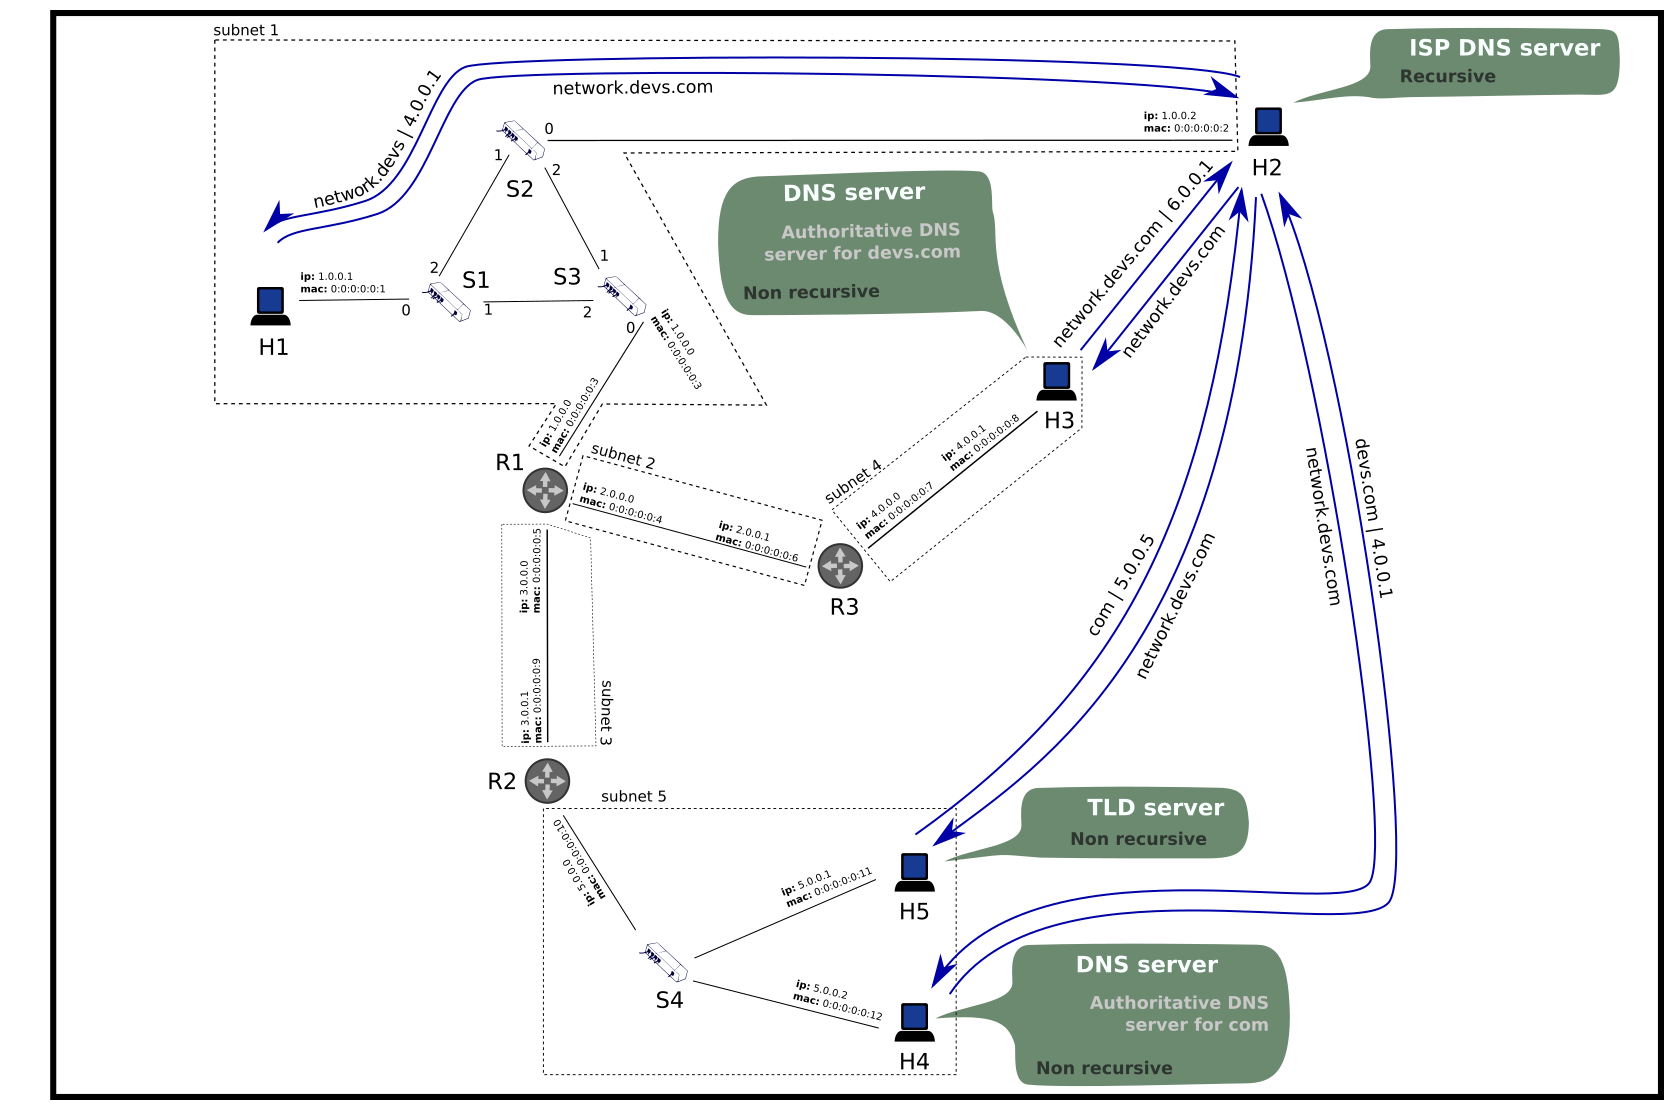
\includegraphics[width = 1.0\textwidth]{img/png/scenario.png}
    \caption{Escenario implementado.}
    \label{figure: case study}
\end{figure}\todo[]{corregir el gráfico: tamaño de los ip y macs, agregar MAC de los switches, e interfaces del switch que falta, cambiar todo a español y cambiar no recursivo por iterativo}

\section{Resultados}
\section{Conclusiones}
\section{Trabajo futuro}

\section{References}
\bibliographystyle{plain}
\bibliography{references}

\end{document}
